% Soubory musí být v kódování, které je nastaveno v příkazu \usepackage[...]{inputenc}

\documentclass[%        Základní nastavení
%  draft,    				  % Testovací překlad
  11pt,       				% Velikost základního písma je 12 bodů
  a4paper,    				% Formát papíru je A4
  oneside,      			% Jednostranný tisk
  %twoside,      			% Dvoustranný tisk (kapitoly a další důležité části tedy začínají na lichých stranách)
	unicode,						% Záložky a metainformace ve výsledném  PDF budou v kódování unicode
]{report}				    	% Dokument třídy 'zpráva', vhodná pro sazbu závěrečných prací s kapitolami

\usepackage[utf8]		  %	Kódování zdrojových souborů je UTF-8
	{inputenc}					% Balíček pro nastavení kódování zdrojových souborů

\usepackage[				% Nastavení geometrie stránky
	bindingoffset=10mm,		% Hřbet pro vazbu
	hmargin={25mm,18mm},	% Vnitřní a vnější okraj
  %hmargin={25mm,25mm},	% Vnitřní a vnější okraj
	%vmargin={25mm,34mm},	% Horní a dolní okraj
  vmargin={20mm,25mm},	% Horní a dolní okraj
	footskip=15mm,			  % Velikost zápatí
	nohead,					      % Bez záhlaví
	marginparsep=2mm,		  % Vzdálenost marginálií
	marginparwidth=18mm,	% Šířka marginálií
]{geometry}

\setcounter{tocdepth}{3}

\usepackage{sectsty}
	%přetypuje nadpisy všech úrovní na bezpatkové, kromě \chapter, která je přenastavena zvlášť v thesis.sty
	\allsectionsfont{\sffamily}

\usepackage{graphicx} % Balíček 'graphicx' pro vkládání obrázků
											% Nutné pro vložení logotypů školy a fakulty

\usepackage[          % Balíček 'acronym' pro sazby zkratek a symbolů
	nohyperlinks				% Nebudou tvořeny hypertextové odkazy do seznamu zkratek
]{acronym}						
											% Nutné pro použití prostředí 'acronym' balíčku 'thesis'

\usepackage[
	breaklinks=true,		% Hypertextové odkazy mohou obsahovat zalomení řádku
	hypertexnames=false % Názvy hypertext. odkazů budou tvořeny nezávisle na názvech TeXu
]{hyperref}						% Balíček 'hyperref' pro sazbu hypertextových odkazů
											% Nutné pro použití příkazu 'pdfsettings' balíčku 'thesis'

\usepackage{pdfpages} % Balíček umožňující vkládat stránky z PDF souborů
                      % Nutné při vkládání titulních listů a zadání přímo
                      % ve formátu PDF z informačního systému

\usepackage{enumitem} % Balíček pro nastavení mezerování v odrážkách
  \setlist{topsep=0pt,partopsep=0pt,noitemsep} % konkrétní nastavení

\usepackage{cmap} 		% Balíček cmap zajišťuje, že PDF vytvořené `pdflatexem' je
											% plně "prohledávatelné" a "kopírovatelné"

%\usepackage{upgreek}	% Balíček pro sazbu stojatých řeckých písmem
											%% např. stojaté pí: \uppi
											%% např. stojaté mí: \upmu (použitelné třeba v mikrometrech)
											%% pozor, grafická nekompatibilita s fonty typu Computer Modern!
                      
%\usepackage{amsmath} %balíček pro sabu náročnější matematiky                 

\usepackage{dirtree}	% sazba adresářové struktury
                      % vhodné pro prezentaci obsahu elektronické přílohy (např. CD)
                    
\usepackage{indentfirst}
\usepackage{pdflscape}
\usepackage{float}
\usepackage[formats]{listings}	% Balíček pro sazbu zdrojových textů
\lstset{              % nastavení
%	Definice jazyka použitého ve výpisech
%    language=[LaTeX]{TeX},	% LaTeX
%	language={Matlab},		% Matlab
	language={C},           % jazyk C
    basicstyle=\ttfamily,	% definice základního stylu písma
    tabsize=2,			% definice velikosti tabulátoru
    inputencoding=utf8,         % pro soubory uložené v kódování UTF-8
		columns=fixed,  %fixed nebo flexible,
		fontadjust=true %licovani sloupcu
    extendedchars=true,
    literate=%  definice symbolů s diakritikou
    {á}{{\'a}}1
    {č}{{\v{c}}}1
    {ď}{{\v{d}}}1
    {é}{{\'e}}1
    {ě}{{\v{e}}}1
    {í}{{\'i}}1
    {ň}{{\v{n}}}1
    {ó}{{\'o}}1
    {ř}{{\v{r}}}1
    {š}{{\v{s}}}1
    {ť}{{\v{t}}}1
    {ú}{{\'u}}1
    {ů}{{\r{u}}}1
    {ý}{{\'y}}1
    {ž}{{\v{z}}}1
    {Á}{{\'A}}1
    {Č}{{\v{C}}}1
    {Ď}{{\v{D}}}1
    {É}{{\'E}}1
    {Ě}{{\v{E}}}1
    {Í}{{\'I}}1
    {Ň}{{\v{N}}}1
    {Ó}{{\'O}}1
    {Ř}{{\v{R}}}1
    {Š}{{\v{S}}}1
    {Ť}{{\v{T}}}1
    {Ú}{{\'U}}1
    {Ů}{{\r{U}}}1
    {Ý}{{\'Y}}1
    {Ž}{{\v{Z}}}1
}

%%%%%%%%%%%%%%%%%%%%%%%%%%%%%%%%%%%%%%%%%%%%%%%%%%%%%%%%%%%%%%%%%
%%%%%%      Definice informací o dokumentu             %%%%%%%%%%
%%%%%%%%%%%%%%%%%%%%%%%%%%%%%%%%%%%%%%%%%%%%%%%%%%%%%%%%%%%%%%%%%

% V tomto souboru se nastavují téměř veškeré informace, proměnné mezi studenty:
% jméno, název práce, pohlaví atd.
% Tento soubor je SDÍLENÝ mezi textem práce a prezentací k obhajobě -- netřeba něco nastavovat na dvou místech.

\usepackage[
%%% Z následujících voleb jazyka lze použít pouze jednu
  czech-english,		% originální jazyk je čeština, překlad je anglicky (výchozí)
  %english-czech,	% originální jazyk je angličtina, překlad je česky
  %slovak-english,	% originální jazyk je slovenština, překlad je anglicky
  %english-slovak,	% originální jazyk je angličtina, překlad je slovensky
%
%%% Z následujících voleb typu práce lze použít pouze jednu
  semestral,		  % semestrální práce (nesází se abstrakty, prohlášení, poděkování) (výchozí)
  %bachelor,			%	bakalářská práce
  %master,			  % diplomová práce
  %treatise,			% pojednání o disertační práci
  %doctoral,			% disertační práce
%
%%% Z následujících voleb zarovnání objektů lze použít pouze jednu
%  left,				  % rovnice a popisky plovoucích objektů budou zarovnány vlevo
	center,			    % rovnice a popisky plovoucích objektů budou zarovnány na střed (vychozi)
%
]{thesis}   % Balíček pro sazbu studentských prací


%%% Jméno a příjmení autora ve tvaru
%  [tituly před jménem]{Křestní}{Příjmení}[tituly za jménem]
% Pokud osoba nemá titul před/za jménem, smažte celý řetězec '[...]'
\author[Bc.]{Filip}{Paul}

%%% Identifikační číslo autora (VUT ID)
\butid{211 538}

%%% Pohlaví autora/autorky
% (nepoužije se ve variantě english-czech ani english-slovak)
% Číselná hodnota: 1...žena, 0...muž
\gender{0}

%%% Jméno a příjmení vedoucího/školitele včetně titulů
%  [tituly před jménem]{Křestní}{Příjmení}[tituly za jménem]
% Pokud osoba nemá titul před/za jménem, smažte celý řetězec '[...]'
\advisor[prof.\ Dr.\ Ing.]{Zdeněk}{Kolka}[...]

%%% Jméno a příjmení oponenta včetně titulů
%  [tituly před jménem]{Křestní}{Příjmení}[tituly za jménem]
% Pokud osoba nemá titul před/za jménem, smažte celý řetězec '[...]'
% Nastavení oponenta se uplatní pouze v prezentaci k obhajobě;
% v případě, že nechcete, aby se na titulním snímku prezentace zobrazoval oponent, pouze příkaz zakomentujte;
% u obhajoby semestrální práce se oponent nezobrazuje (jelikož neexistuje)
% U dizertační práce jsou typicky dva až tři oponenti. Pokud je chcete mít na titulním slajdu, prosím ručně odkomentujte a upravte jejich jména v definici "VUT title page" v souboru thesis.sty.
\opponent[doc.\ Mgr.]{Křestní}{Příjmení}[Ph.D.]

%%% Název práce
%  Parametr ve složených závorkách {} je název v originálním jazyce,
%  parametr v hranatých závorkách [] je překlad (podle toho jaký je originální jazyk).
%  V případě, že název Vaší práce je dlouhý a nevleze se celý do zápatí prezentace, použijte příkaz
%  \def\insertshorttitle{Zkác.\ náz.\ práce}
%  kde jako parametr vyplníte zkrácený název. Pokud nechcete zkracovat název, budete muset předefinovat,
%  jak se vytváří patička slidu. Viz odkaz: https://bit.ly/3EJTp5A
\title[Title of Student's Thesis]{Výrobní tester}

%%% Označení oboru studia
%  Parametr ve složených závorkách {} je název oboru v originálním jazyce,
%  parametr v hranatých závorkách [] je překlad
\specialization[Teleinformatics]{Teleinformatika}

%%% Označení ústavu
%  Parametr ve složených závorkách {} je název ústavu v originálním jazyce,
%  parametr v hranatých závorkách [] je překlad
%\department[Department of Control and Instrumentation]{Ústav automatizace a měřicí techniky}
%\department[Department of Biomedical Engineering]{Ústav biomedicínského inženýrství}
%\department[Department of Electrical Power Engineering]{Ústav elektroenergetiky}
%\department[Department of Electrical and Electronic Technology]{Ústav elektrotechnologie}
%\department[Department of Physics]{Ústav fyziky}
%\department[Department of Foreign Languages]{Ústav jazyků}
%\department[Department of Mathematics]{Ústav matematiky}
%\department[Department of Microelectronics]{Ústav mikroelektroniky}
\department[Department of Radio Electronics]{Ústav radioelektroniky}
%\department[Department of Theoretical and Experimental Electrical Engineering]{Ústav teoretické a experimentální elektrotechniky}
%\department[Department of Telecommunications]{Ústav telekomunikací}
%\department[Department of Power Electrical and Electronic Engineering]{Ústav výkonové elektrotechniky a elektroniky}

%%% Označení fakulty
%  Parametr ve složených závorkách {} je název fakulty v originálním jazyce,
%  parametr v hranatých závorkách [] je překlad
%\faculty[Faculty of Architecture]{Fakulta architektury}
\faculty[Faculty of Electrical Engineering and~Communication]{Fakulta elektrotechniky a~komunikačních technologií}
%\faculty[Faculty of Chemistry]{Fakulta chemická}
%\faculty[Faculty of Information Technology]{Fakulta informačních technologií}
%\faculty[Faculty of Business and Management]{Fakulta podnikatelská}
%\faculty[Faculty of Civil Engineering]{Fakulta stavební}
%\faculty[Faculty of Mechanical Engineering]{Fakulta strojního inženýrství}
%\faculty[Faculty of Fine Arts]{Fakulta výtvarných umění}
%
%Nastavení logotypu (v hranatych zavorkach zkracene logo, ve slozenych plne):
\facultylogo[logo/FEKT_zkratka_barevne_PANTONE_CZ]{logo/UTKO_color_PANTONE_CZ}

%%% Rok odevzdání práce
\graduateyear{2023}
%%% Akademický rok odevzdání práce
\academicyear{2022/23}

%%% Datum obhajoby (uplatní se pouze v prezentaci k obhajobě)
\date{11.\,11.\,1980} 

%%% Místo obhajoby
% Na titulních stránkách bude automaticky vysázeno VELKÝMI písmeny (pokud tyto stránky sází šablona)
\city{Brno}

%%% Abstrakt
\abstract[%
Překlad abstraktu
(v~angličtině, pokud je originálním jazykem čeština či slovenština; v~češtině či slovenštině, pokud je originálním jazykem angličtina)
]{%
Abstrakt práce v~originálním jazyce
}

%%% Klíčová slova
\keywrds[%
Překlad klíčových slov
(v~angličtině, pokud je originálním jazykem čeština či slovenština; v~češtině či slovenštině, pokud je originálním jazykem angličtina)
]{%
Klíčová slova v~originálním jazyce
}

%%% Poděkování
\acknowledgement{%
Rád bych poděkoval vedoucímu diplomové práce
panu Prof. Dr. Ing. Zdeňku Kolkovi za odborné vedení,
konzultace, trpělivost a~podnětné návrhy k~práci.
}%  % do tohoto souboru doplňte údaje o sobě, druhu práce, názvu...

%%%%%%%%%%%%%%%%%%%%%%%%%%%%%%%%%%%%%%%%%%%%%%%%%%%%%%%%%%%%%%%%%%%%%%%%

%%%%%%%%%%%%%%%%%%%%%%%%%%%%%%%%%%%%%%%%%%%%%%%%%%%%%%%%%%%%%%%%%%%%%%%%
%%%%%%     Nastavení polí ve Vlastnostech dokumentu PDF      %%%%%%%%%%%
%%%%%%%%%%%%%%%%%%%%%%%%%%%%%%%%%%%%%%%%%%%%%%%%%%%%%%%%%%%%%%%%%%%%%%%%
%% Při načteném balíčku 'hyperref' lze použít příkaz '\pdfsettings':
%\pdfsettings
%  Nastavení polí je možné provést také ručně příkazem:
%\hypersetup{
%  pdftitle={Název studentské práce},    	% Pole 'Document Title'
%  pdfauthor={Autor studenstké práce},   	% Pole 'Author'
%  pdfsubject={Typ práce}, 						  	% Pole 'Subject'
%  pdfkeywords={Klíčová slova}           	% Pole 'Keywords'
%}
%%%%%%%%%%%%%%%%%%%%%%%%%%%%%%%%%%%%%%%%%%%%%%%%%%%%%%%%%%%%%%%%%%%%%%%
\pdfmapfile{=vafle.map}

%%%%%%%%%%%%%%%%%%%%%%%%%%%%%%%%%%%%%%%%%%%%%%%%%%%%%%%%%%%%%%%%%%%%%%%
%%%%%%%%%%%       Začátek dokumentu               %%%%%%%%%%%%%%%%%%%%%
%%%%%%%%%%%%%%%%%%%%%%%%%%%%%%%%%%%%%%%%%%%%%%%%%%%%%%%%%%%%%%%%%%%%%%%
\setlength{\abovecaptionskip}{2pt} % Chosen fairly arbitrarily
\setlength{\belowcaptionskip}{0pt} % Chosen fairly arbitrarily

\begin{document}
\hypersetup{hidelinks}
\pagestyle{empty} %vypnutí číslování stránek


\includepdf[page = 1]{pdf/student-titulka.pdf}

\tableofcontents

\cleardoublepage\pagestyle{plain}   % zapnutí číslování stránek
%\setcounter{page}{1}

%Pro vkládání kapitol i příloh používejte raději \include než \input
%%% Vložení souboru 'text/uvod.tex' s úvodem
\chapter*{Úvod}
\phantomsection
\addcontentsline{toc}{chapter}{Úvod}

\indent Cílem odborné praxe bylo navrhnout a realizovat
poloautomatizované pracoviště,
které bude schopno naprogramovat a následně ověřit funkčnost
různých desek plošných spojů.
Pracoviště může obsluhovat neodborná osoba, která provádí pouze jednoduché úkony,
ke kterým je instruována pomocí monitoru. Zařízení vyhodnotí zda testovaná
deska vyhovuje všem požadovaným parametrům a následně odešle výsledek testu
do databáze.\\

Vzhledem ke komplexnosti zařízení a rozsahu zprávy o náplni praxe,
je práce koncipována spíše jako uživatelský manuál k zařízení než jako podrobná technická zpráva.\\

Zařízení bylo navrženo a vyrobeno ve spolupráci s firmou Čevor Inovation a.s. A v současné
době zařízení funguje ve výrobním provozu firmy SIEMENS.

%%% Vložení souboru 'text/cile.tex' s úvodem
%%\chapter*{Cíle práce}
\phantomsection
\addcontentsline{toc}{chapter}{Cíle práce}

Konkrétní specifikace cílů, které má autor v~práci vyřešit.
Tato kapitola je \emph{volitelná} -- pokud váš studijní program nevyžaduje zvláštní kapitolu s cíli,
cíle specifikujte v~rámci Úvodu.

%%% Vložení souboru 'text/reseni' s popisem řešení práce
% (rozdělte na více souborů či kapitol, pokud je vhodné)

\chapter{Popis zařízení:}
		Zařízení se skládá z následujících základních částí: STŮL, RACK, INTERFACE, vyměnitelných ADAPTÉRŮ
		a ostatních zařízení připojených do rackového PC. Zařízení je určeno k programování a testování
		desek plošných spojů (dále označováno jako DUT). DUT se vkládá do ADAPTÉRU, kde je nakontaktováno pomocí mechanického
		zavírání a testovacích jehel. Proces je do jisté míry automatizován řídícím softwarem,
		který je popsán v kapitole software. Software předává obsluze pokyny a informace pomocí textu na monitoru. 
		
		\begin{figure}[ht!]
			\centering
			\includegraphics[height = 0.74\textheight]{obrazky/Zapojeni.png}
			\caption{Blokový diagram zapojení pracoviště}
            \label{fig:Blokový diagram zapojení pracoviště}
		\end{figure}
\clearpage
	\section{Stůl}
	Celý systém je zabudován do stolu. Stůl disponuje možností nastavitelnosti výšky celé konstrukce a sklonu desky,
	do které je upevněn INTERFACE a ADAPTÉR. Do stolu je přivedeno napětí 230V,
	které je dále rozvedeno přes proudový chránič do zásuvek pod stolem a RACKU.\\

	\begin{figure}[ht!]
		\begin{minipage}{0.49\textwidth}
			\vspace{-3.3cm}
			\textbf{Nastavení výšky:}\\\\
			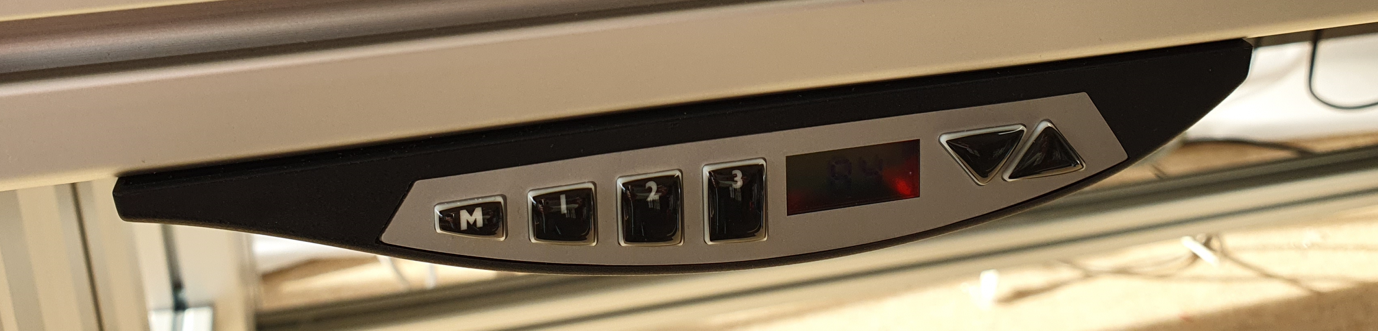
\includegraphics[width = 0.9\textwidth]{obrazky/vyska.png}
            \caption{Nastavení výšky stolu}
			
		\end{minipage}
		\begin{minipage}{0.49\textwidth}
			\textbf{Nastavení sklonu:}\\\\
			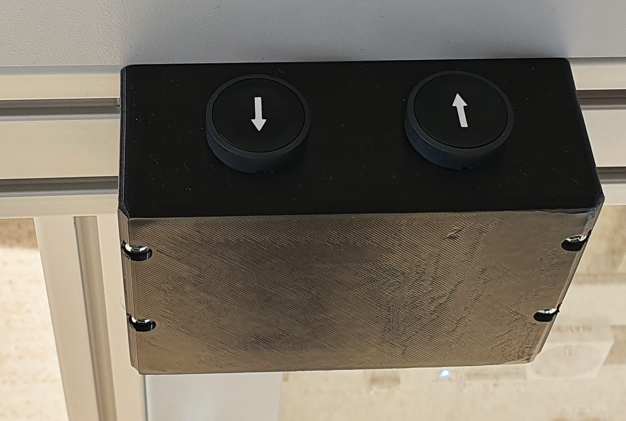
\includegraphics[width = 0.9\textwidth]{obrazky/sklon.png}
            \caption{Nastavení sklonu stolu}
			
		\end{minipage}
	\end{figure}

	\section{Rack}
	Úkolem RACK je poskytnou napájení celému systému pomocí několika galvanicky oddělených zdrojů napětí (viz schéma el. zapojení).
	Je zde umístěn i programovatelný zdroj GWINSTEK GPP-2323 jehož výstupy (kanál 1 a 2)
	jsou vyvedeny do svorek na přední části RACKU pro potřeby kalibrace.
	Dále obsahuje servisní zásuvku a bezpečnostní prvky jako vypínací tlačítko, jističe a proudový chránič.
	Dále je zde umístěn počítač, který celý systém řídí pomocí softwaru popsaného v kapitole SOFTWARE.
    Rack je možné uzamykat pomocí zámku na klíč.

	\section{Interface}
	V interface je umístěna hlavní řídící deska ARRIGO která ovládá a monituruje stav zařízení
	(spínání relátek, identifikace připojeného adaptéru, kontrola zavření víka apod.).
	Dále je zde umístěno několik programátorů (FLASHRUNNER, Segger Flasher PRO, ASIPROG a SCANBOOSTERII boundary scan).
	Za účelem externího programování (bez adaptéru) je vyveden výstup z FLASHRUNNER do konektoru CANNON 25
    na krabici (viz schéma el. zapojení).

	\section{Adaptér}
	Do interface je možno připojit adaptér pomocí propojení přes 170 pinový blok a zaaretování mechanickou pákou.
	ADAPTÉR obsahuje jehlové pole určené k nakontaktování na testpointy DUT,
	mechanické zavírání s detekcí správného založení desky a frézku ke značení testovaných desek.
	Každý adaptér dále obsahuje minimálně jednu relé kartu pro přivedení příslušných signálů na testpointy.
    V současné době je k dispozici 5 připojitelných adaptérů, které jsou schopny otestovat
    22 různých DUT.\\

    V některých složitějších adaptérech lze najít hardware dedikovaný danému provedení DUT. U některých DUT se například
    pro zákaznické čipy používá speciální přídavný hardware. Dále je v některých adaptérech možné najít optické vlákna
    s označením neohýbat. Každý adaptér má dále ve své přední části umístěny signalizační LED.

	\begin{figure}[ht!]
		\begin{minipage}{0.49\textwidth}
			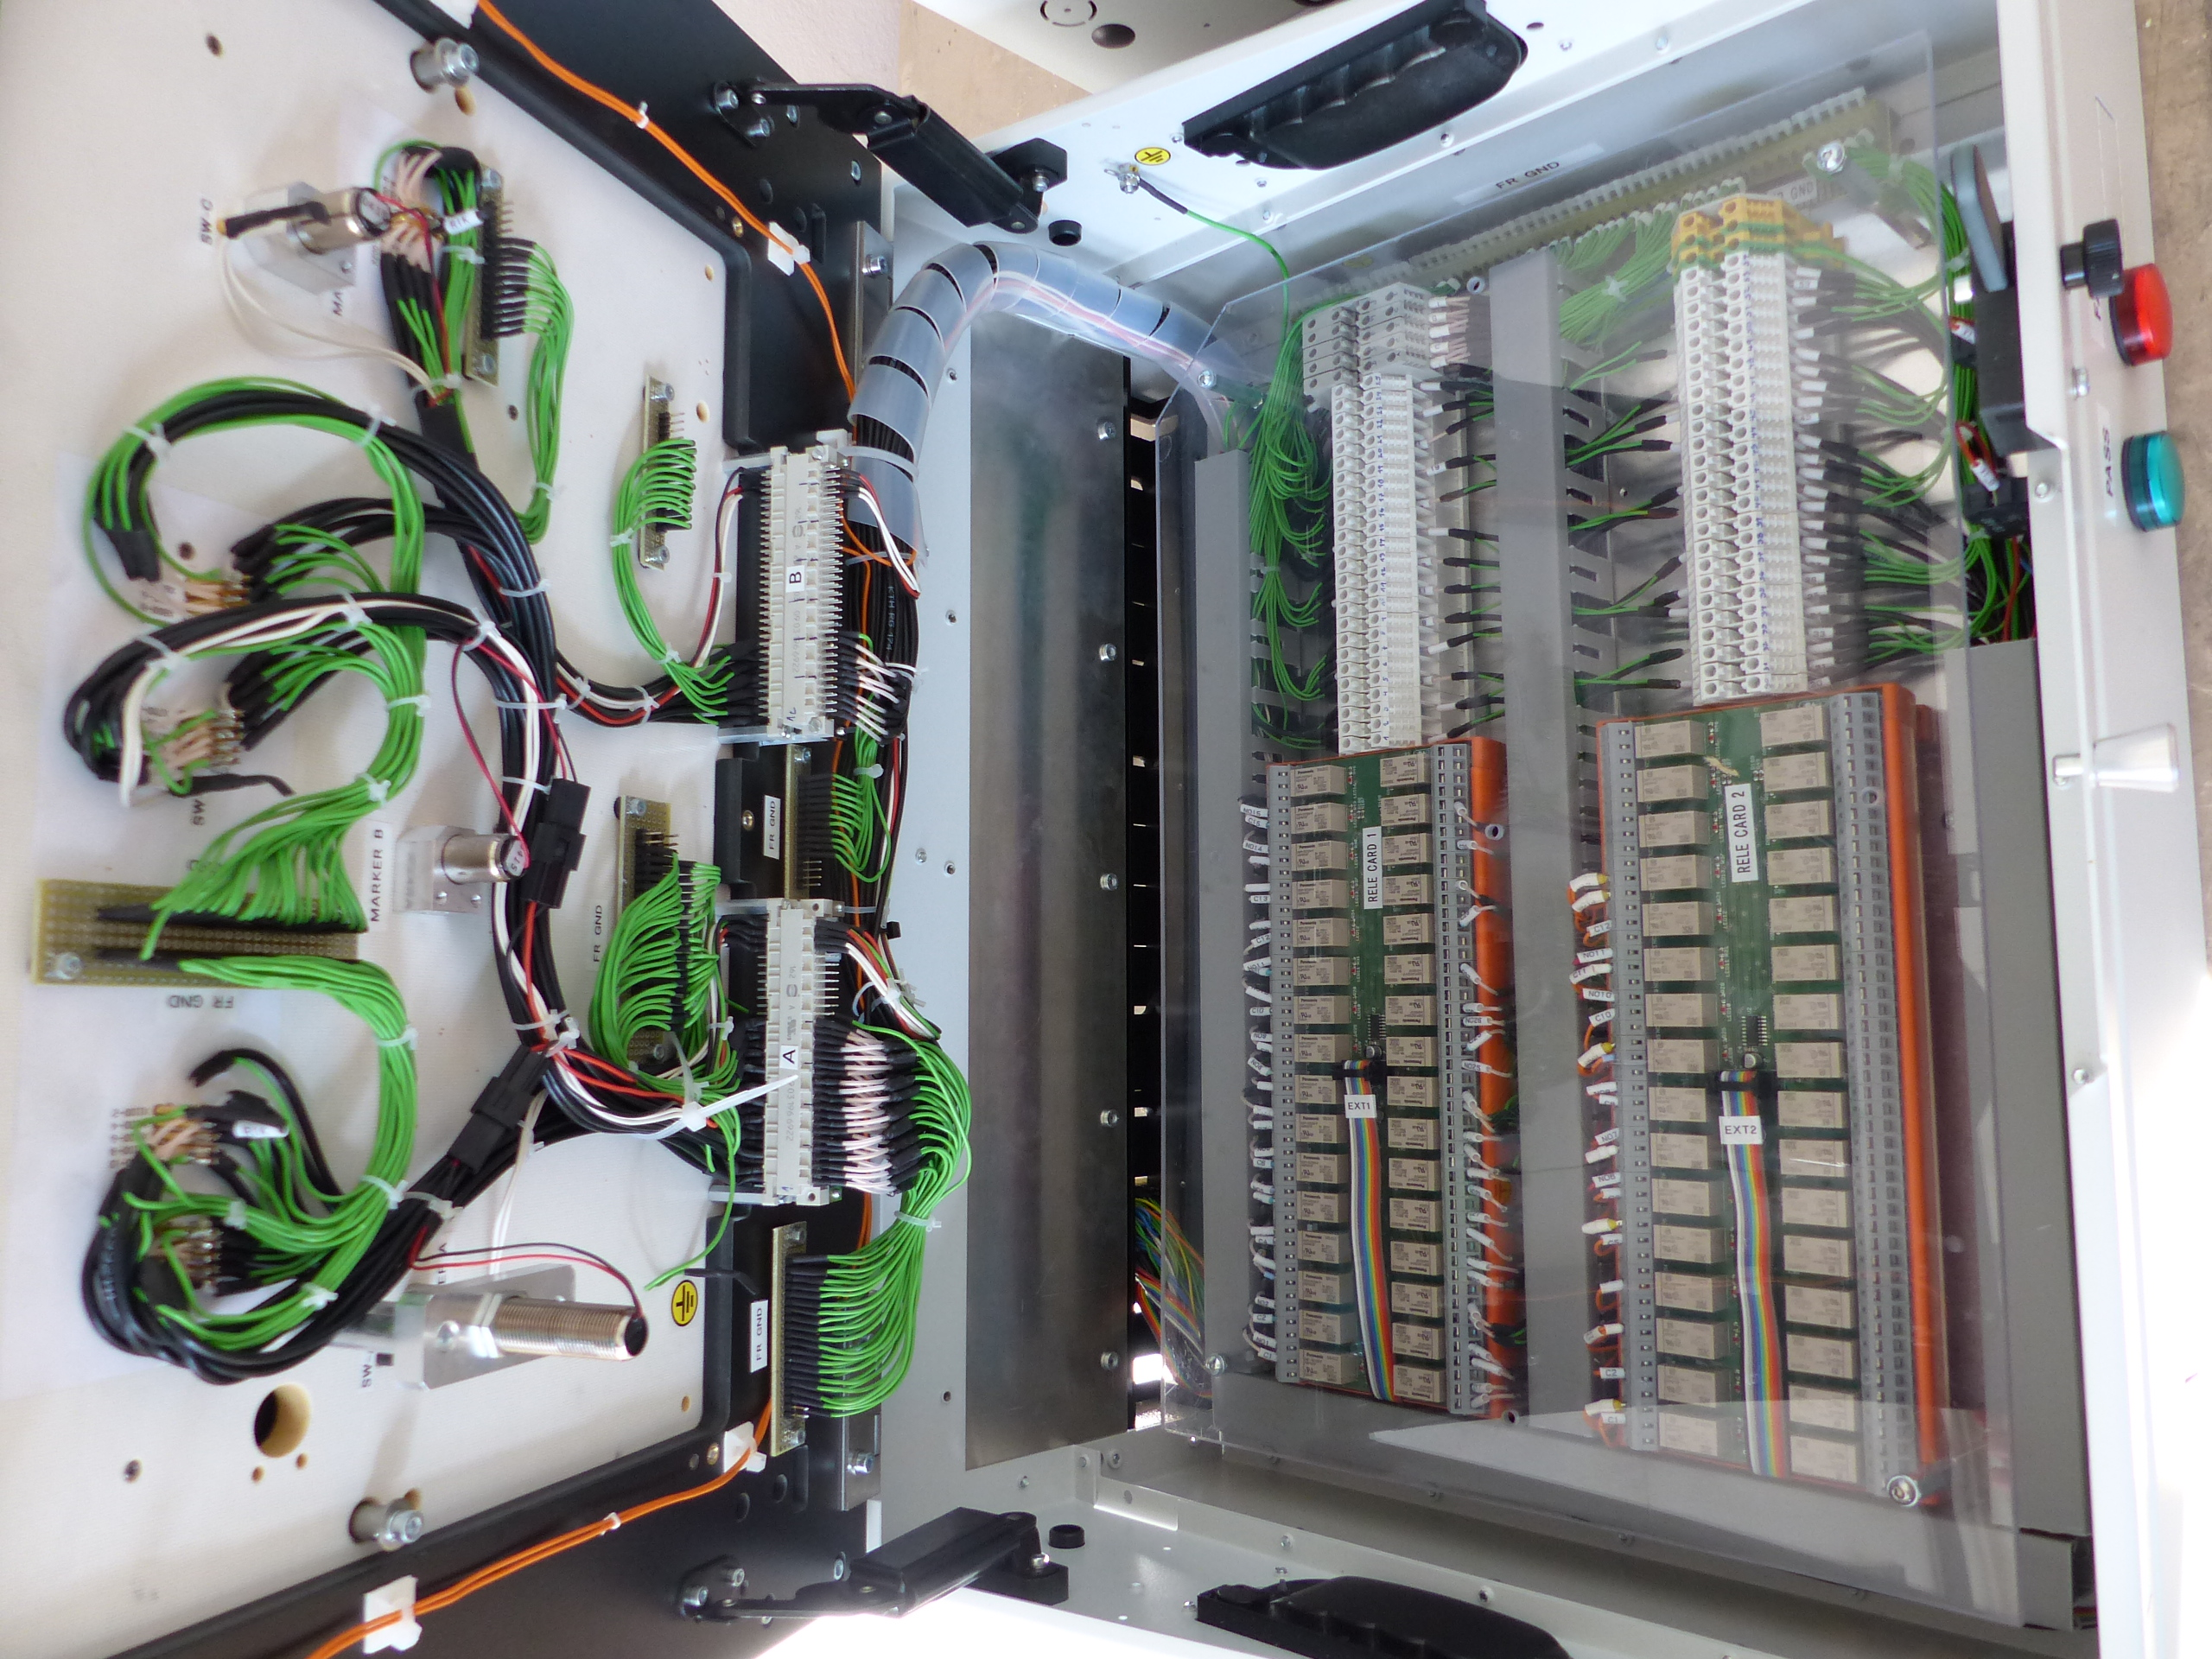
\includegraphics[width = \textwidth ,angle = -90]{obrazky/ADAPTER_INSIGHT.jpg}
            \caption{Vnitřní zapojení adaptéru}
			
		\end{minipage}
		\begin{minipage}{0.49\textwidth}
			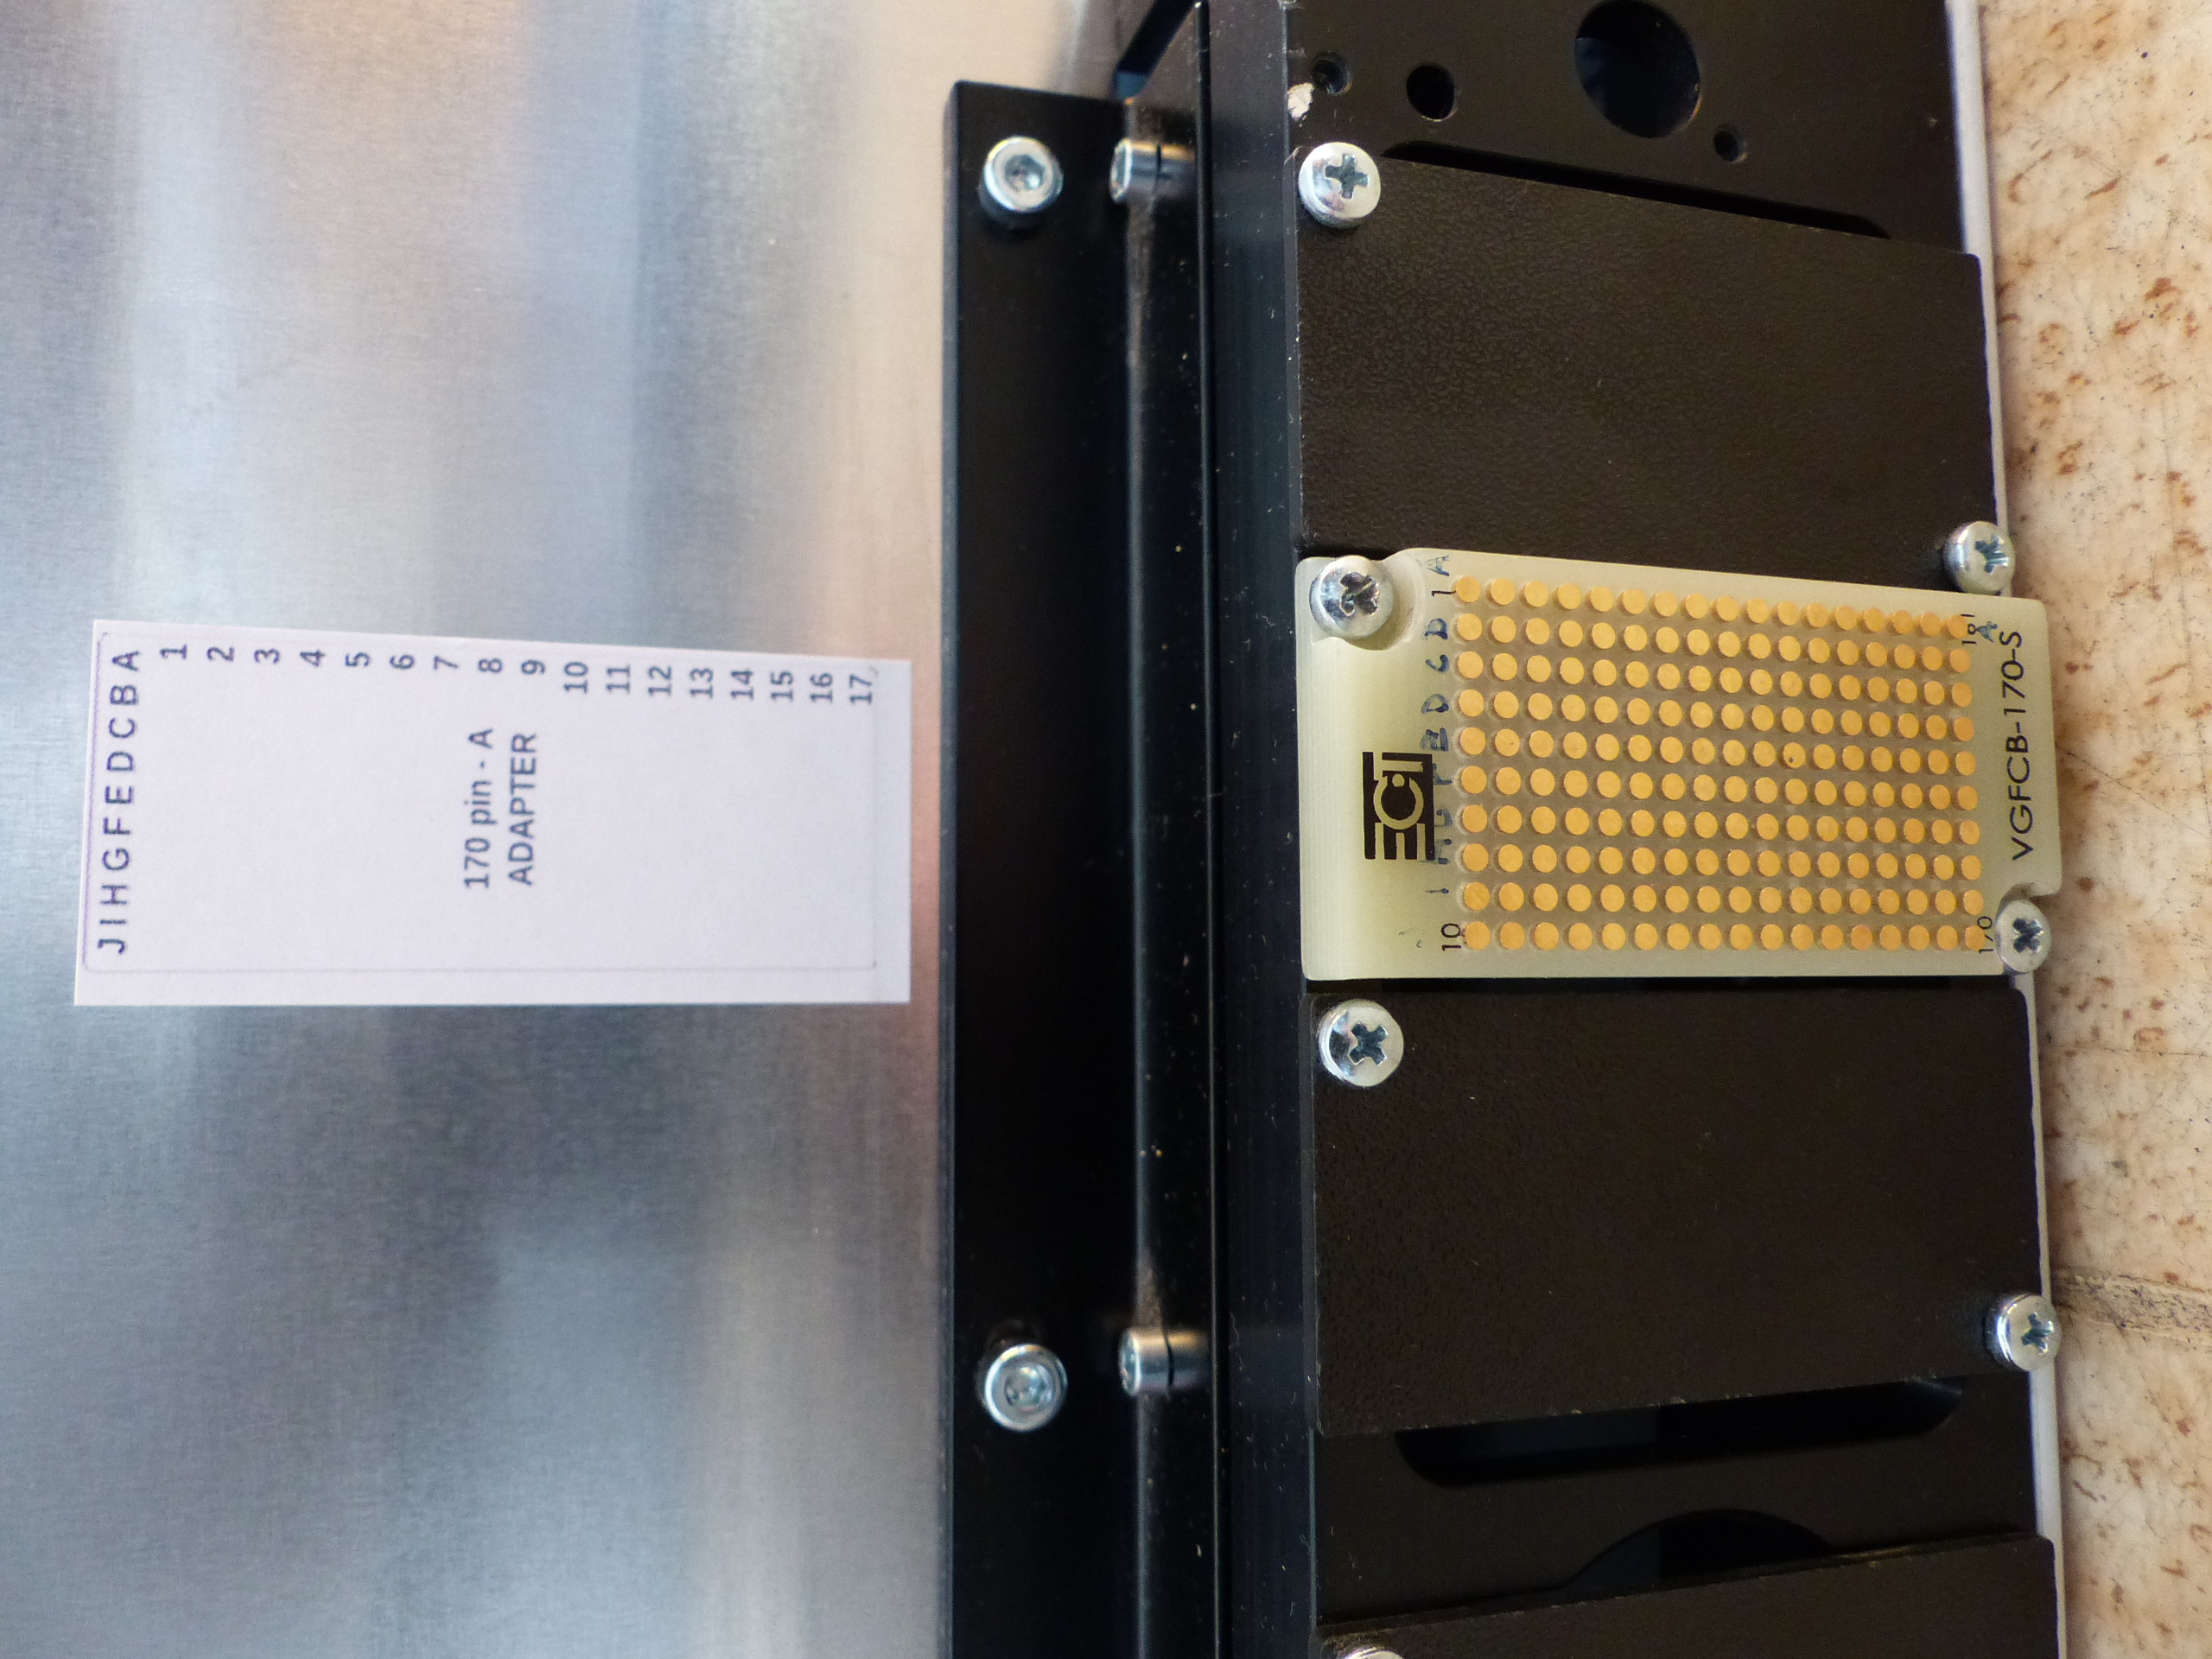
\includegraphics[width = \textwidth, angle = -90]{obrazky/170pin.JPG}
			\caption{Propojovací 170-ti pinový konektor}
		\end{minipage}
	\end{figure}


    \subsection{Výměna adaptérů:}
	Před výměnou adaptéru je doporučeno vypnout software a ujistit se, že neprobíhají žádné testy. Po vypnutí ovládacího 
	softwaru lze bezpečně stávající adaptér odebrat a připojit nový.\\


	\begin{minipage}{0.5\textwidth}
		\begin{enumerate}
			\item Pokud běží ovládací software, počkejte na dokončení testů a software vypněte.
			\item Odaretujte adaptér pomocí aretační páky
			\item Adaptér nadzvedněte tak, aby došlo k vyháknutí adaptéru z háků za které je zachycen.
			\item Do háků vložte nový adaptér
			\item Zaaretujte adaptér pomocí aretační páky
		\end{enumerate}
	\end{minipage}
	\hfill
	\begin{minipage}{0.4\textwidth}
		\begin{figure}[H]
			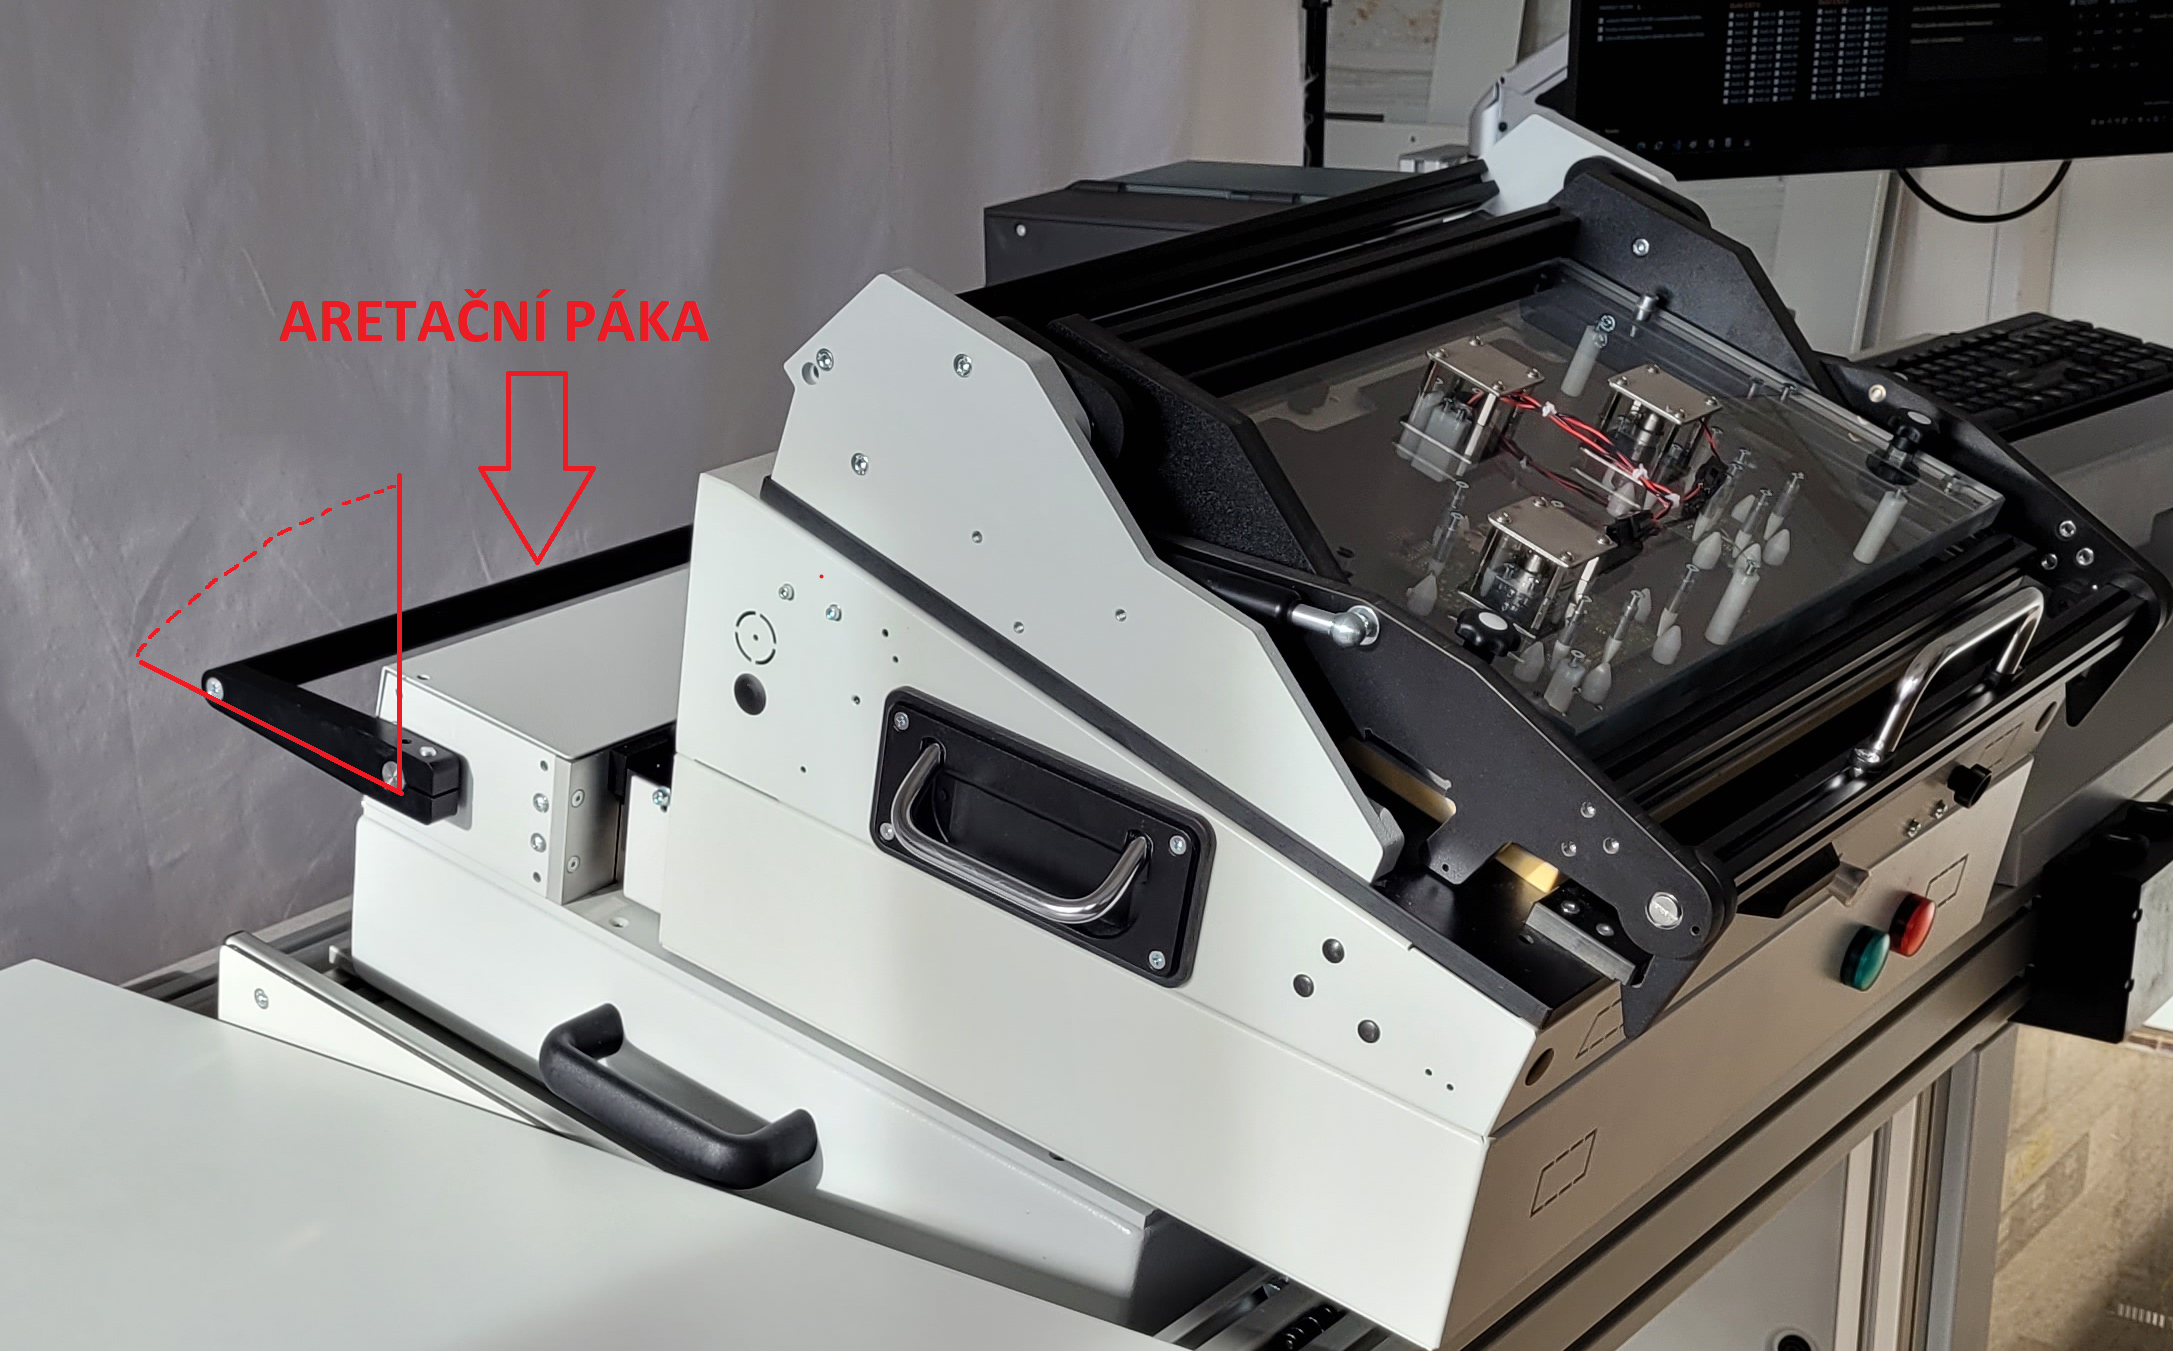
\includegraphics[width = \textwidth]{obrazky/aretacni_paka.png}
            \caption{Aretační páka}
		\end{figure}
	\end{minipage}

% 
\chapter{Obsluha zařízení:}
\section{Pracovní postup:}
	Pracovní postup by se dal shrnout do následujících bodů:

	\begin{enumerate}
		\item Přihlaste se pomocí přiložení uživatelské karty
		\item Naskenujte číslo zakázky
		\item Naskenujte Sériové číslo
		\item Vložte DUT do pozice zobrazené na monitoru\\
        Z důvodu snížení rizika opotřebení testovacích jehel je doporučeno vkládat do pozic, kde není připojena DUT záslepky viz. obrázek níže.
        \begin{figure}[ht!]
            \centering
            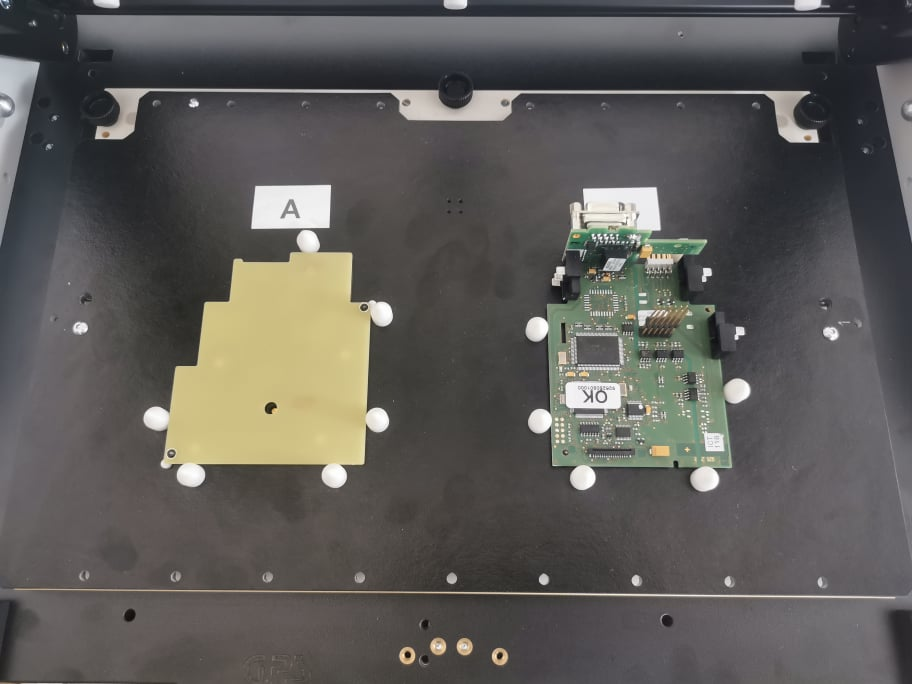
\includegraphics[width = 0.5\textwidth]{obrazky/adapt_zaslepka.jpg}
            \caption{Záslepky pro zakládání DUT do adaptéru}
        \end{figure}
    
		\item Počkejte na dokončení testu
		\item Vyjměte DUT
		\item Postup opakujte od bodu 3.
		\end{enumerate}

	Pro každý bod je obsluha vyzvána k příslušnému postupu pomocí textu na monitoru.
	Dále se může celý systém nacházet v různých chybových stavech. Pokud je chybový stav detekován,
	tak se na obrazovce monitoru zobrazí příslušná chybová hláška o vzniklé chybě a obsluha nebude moci provádět další testy
	až do odstranění chyby. Podrobnější informace naleznete v části SOFTWARE.

\chapter{Software}
Ovládací software lze používat v módu standardního a Admin uživatele.
Mezi jednotlivými módy se lze přepínat buď přiložením Administrátorské RFID karty a nebo
přihlášením pomocí jména "ADMIN" a příslušného hesla. Následující část je věnována módu standardního uživatele.
\section{Standardní uživatel}
Po spuštění programu se zobrazí následující obrazovka.
Program je rozdělen do dvou hlavních sekcí "Volba testované desky" a  "Tester". Přestože je v softwaru 
jasně viditelné logo SIEMENS, z důvodu posedlosti firmy SIEMENS svými logy,
tak celý software byl vytvořen firmou Čevor Innovation a.s.

\begin{figure}[ht!]
	\centering
	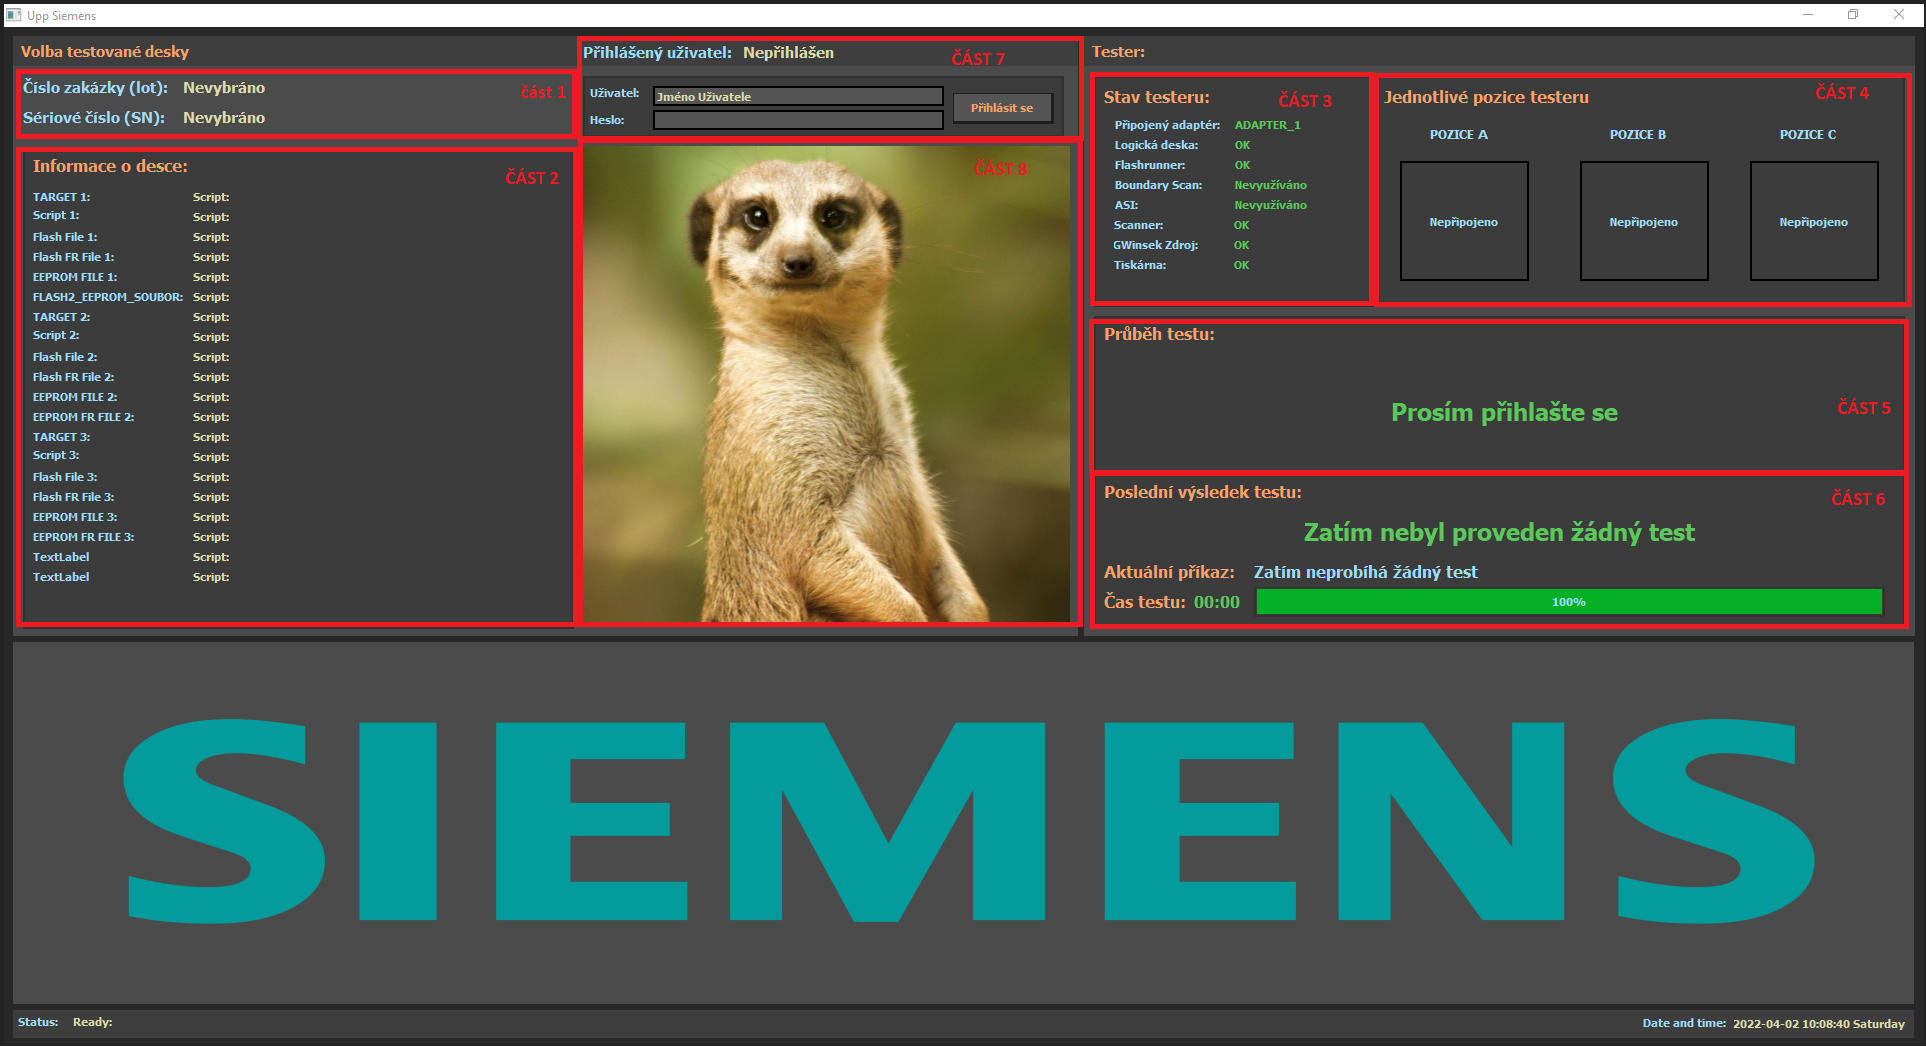
\includegraphics[width = 1\textwidth]{obrazky/LOGIN_EDITED.png}
    \caption{Obrazovka po spuštění programu}
\end{figure}

\subsection{Sekce volba testované desky}
V této sekci jsou zobrazeny v části 1 a 2. informace o právě zvoleném DUT (po zapnutí programu není vybráno žádné DUT). V části 7 
lze nalézt informace o právě přihlášeném uživateli a v části 8. se po přihlášení a naskenování správného
kódu zobrazí foto pro zvolené DUT.

\subsection{Sekce Tester}
V této sekci se v části 3 nacházejí aktuální informace o stavu testeru.
Tester provádí kontinuálně sebekontrolu a výsledky se zobrazují v části 3.
V části 4 jsou zobrazeny jednotlivé pozice připojeného adaptéru, které zobrazují,
zda je nebo není připojena DUT. V části 5 a 6 jsou zobrazovány pokyny obsluze a výsledky aktuálního testu.
Po spuštění programu by se měl zobrazovat pokyn "Prosím přihlaste se".

\clearpage

\section{Software - Obsluha testeru}

\subsection{Přihlášení obsluhy}
Přihlášení obsluhy se provádí pomocí vložení uživatelské karty do slotu pro uživatelské karty. Případně je možné
se přihlásit správnou kombinací jména a hesla v části 7.
V případě, že dojde k přihlášení uživatele, který má v systému uloženou fotografii, tak se změní obrázek surikaty
na obrázek uživatele. V případě, že uživatel nemá uloženou fotografii, tak se bude uživatel muset spokojit
s obrázkem surikaty případně jiného zvířete. 
Po přihlášení by obsluha měla být vyzvána v části 5 k naskenování čísla zakázky.

\subsection{Skenování čísla zakázky:}
Na stole je umístěna ruční čtečka čárových kódů, pomocí které obsluha načte číslo zakázky.
Po načtení čísla zakázky by obsluha měla být vyzvána k naskenování Sériového čísla.

\section{Skenování Sériového čísla:}
Po naskenování čísla zakázky by už měly být dostupné informace o DUT
(foto a informace v levé části programu na Obr.\ref{fig: informace o DUT})
\begin{figure}[ht!]
	\centering
	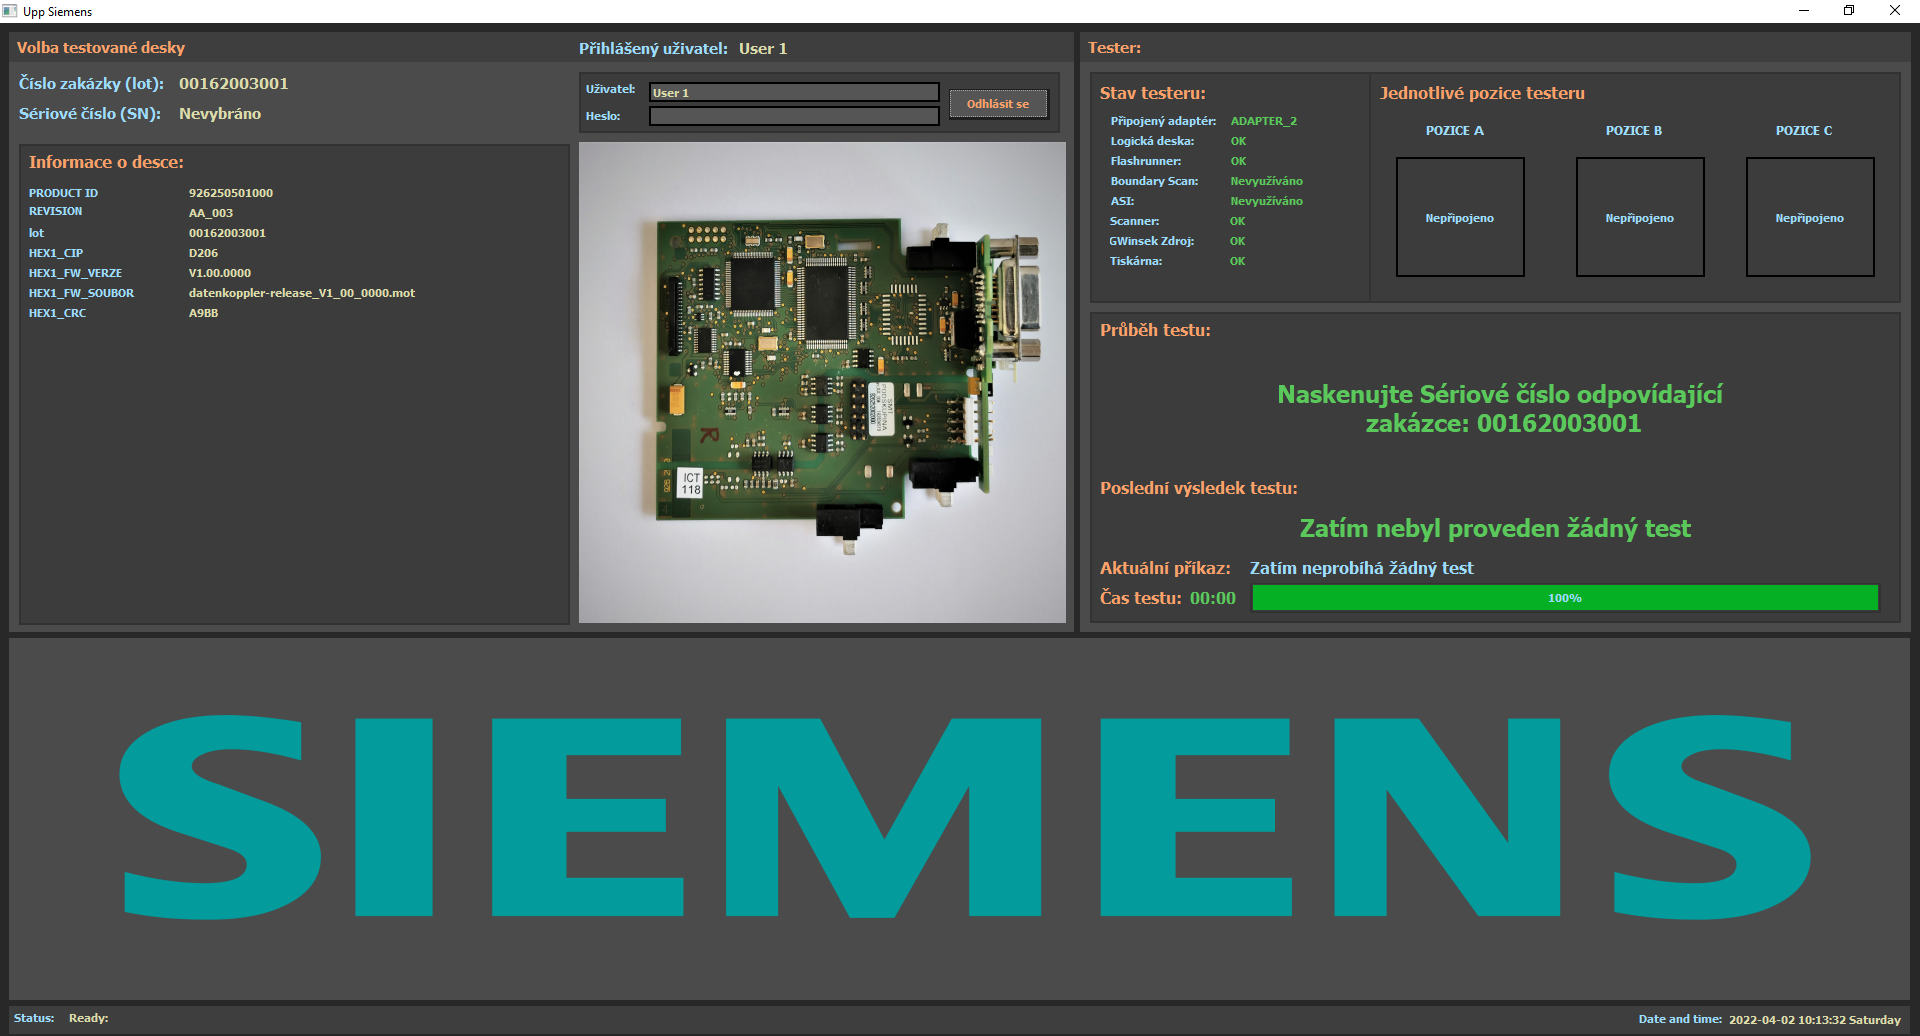
\includegraphics[width = 1\textwidth]{obrazky/SCAN_SN.PNG}
    \caption{Informace o DUT}
    \label{fig: informace o DUT}
\end{figure}

Obdobně jako při skenování čísla zakázky naskenuje obsluha sériové číslo.
Po načtení sériového čísla by obsluha měla být vyzvána k vložení DUT do správné pozice.
V případě, že DUT nemá sériové číslo je možné povolit testování bez sériového čísla v módu ADMIN.

\clearpage
\subsection{Vložení desky do správné pozice:}
Obsluha je nyní vyzvána k založení desky do pozice X a zavření víka.
Zde je navíc graficky znázorněno v části "Jednotlivé pozice testeru", kam má obsluha desku vložit.
Zde může nastat několik různých situací.

\begin{figure}[ht!]
	\begin{minipage}{0.32\textwidth}
		\textbf{Žádné DUT není založeno:}\\\\
		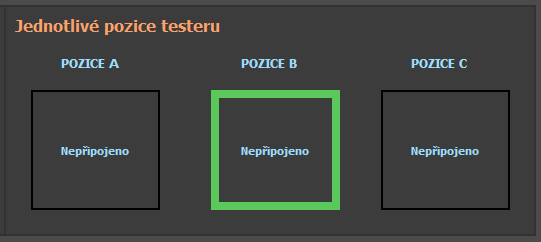
\includegraphics[width = 0.9\textwidth]{obrazky/NO_BOARD.PNG}
		
	\end{minipage}
    \hfill
	\begin{minipage}{0.32\textwidth}
		\textbf{DUT je založeno správně:}\\\\\\
		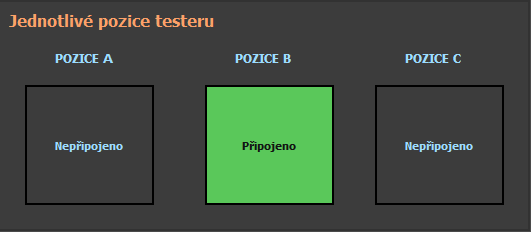
\includegraphics[width = 0.9\textwidth]{obrazky/OK_BOARD.PNG}
		
	\end{minipage}
    \hfill
	\begin{minipage}{0.32\textwidth}
		\textbf{DUT je založeno nesprávně:}\\\\
		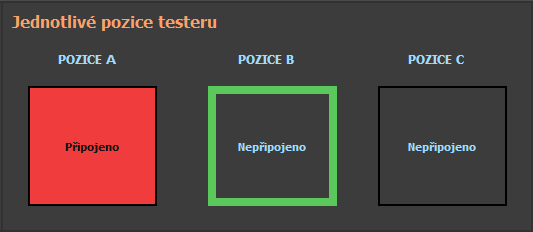
\includegraphics[width = 0.9\textwidth]{obrazky/BAD_BOARD.PNG}
		
	\end{minipage}
    \caption{Identifikace správné pozice DUT}
\end{figure}

Po vložení desky do správné pozice, spustí se testovací procedura pro zvolené DUT
a obsluha je vyzvána k čekání na dokončení testu.
Průběh testu je možno sledovat zde:
\begin{figure}[ht!]
	\centering
	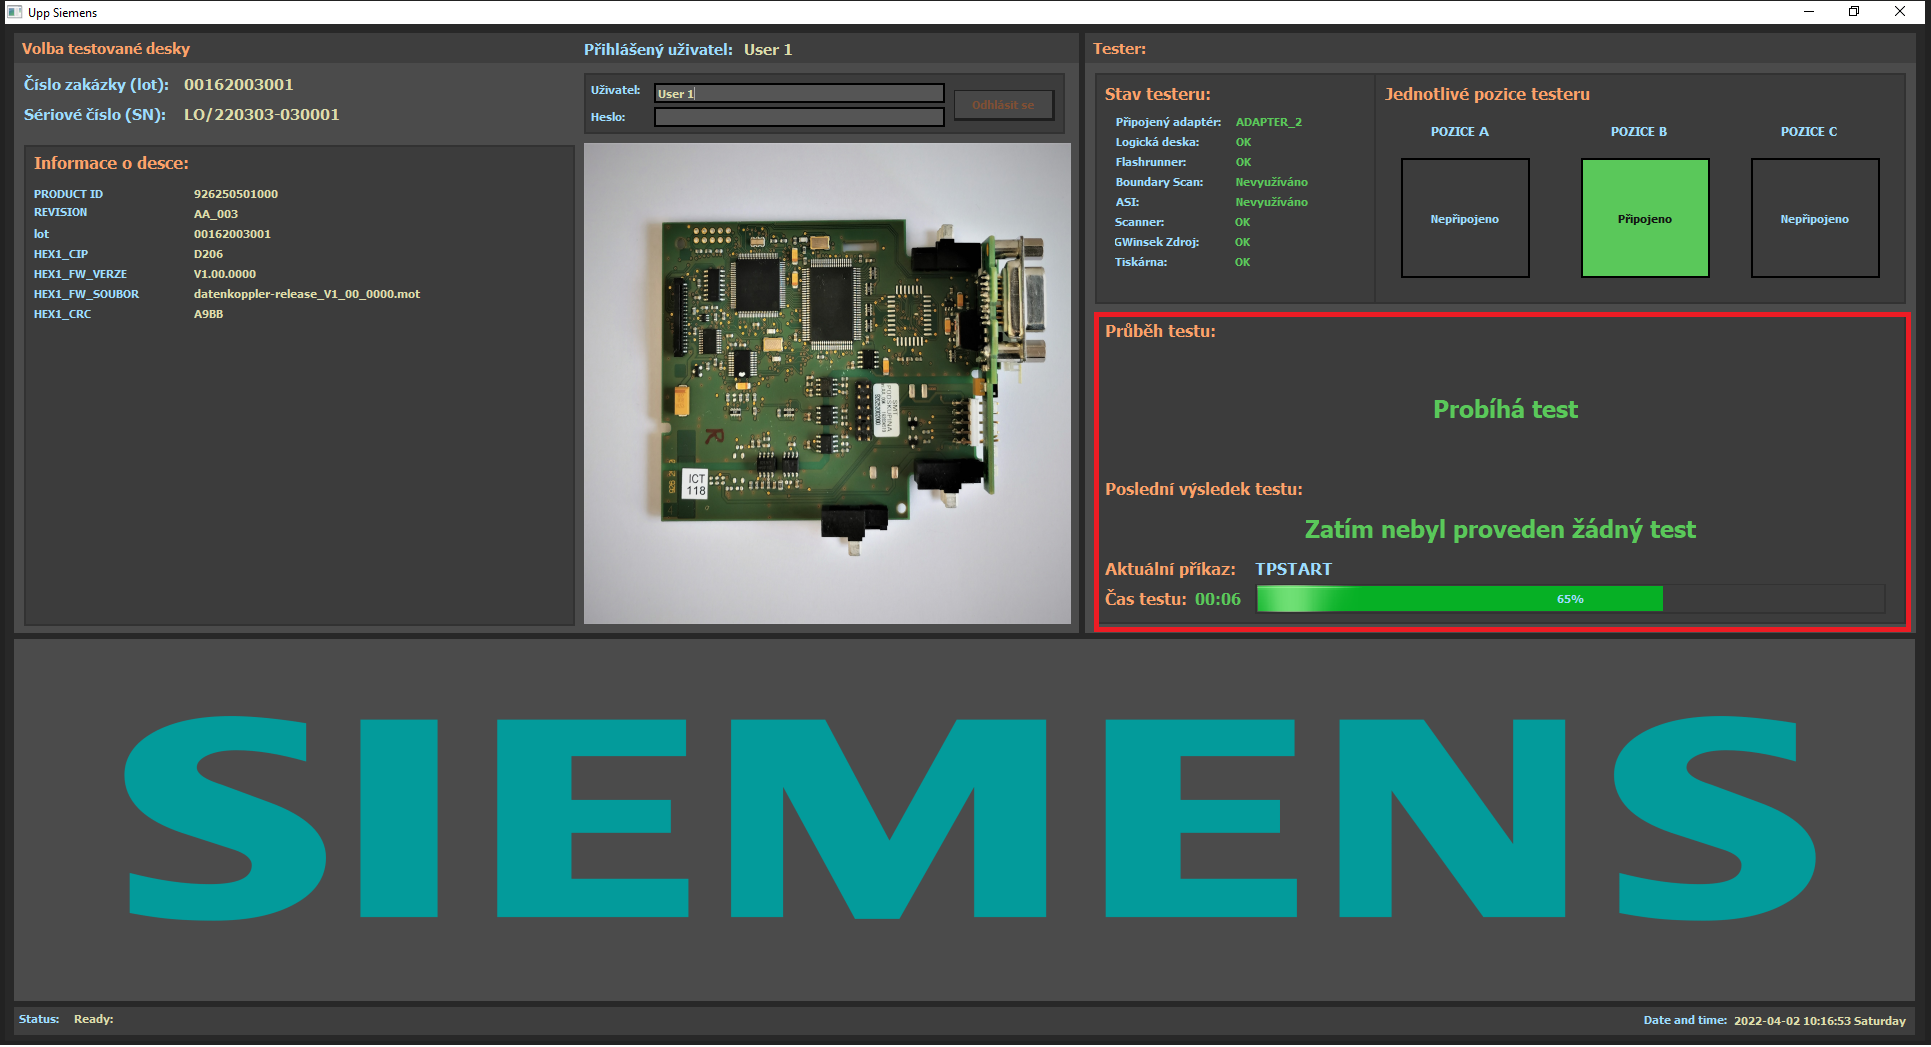
\includegraphics[width = 1\textwidth]{obrazky/TEST_START_EDITED.PNG}
    \caption{Průběh testu}
\end{figure}

\clearpage
\subsection{Dokončení testu:}
Po dokončení testu je v závislosti na výsledku testu obsluha informována o dalším postupu.

\begin{enumerate}
	\item \textbf{Test byl dokončen s výsledkem PASS:}
	\begin{figure}[ht!]
		\centering
		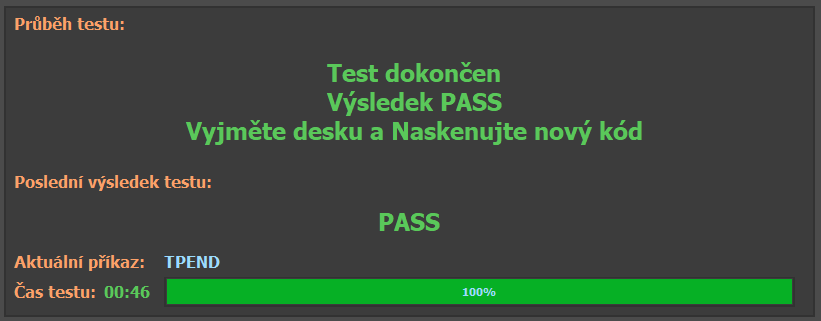
\includegraphics[height = 0.2\textheight]{obrazky/PASS_EDITED.PNG}
	\end{figure}

	\item \textbf{Test byl dokončen s výsledkem FAIL:}
	\begin{figure}[ht!]
		\centering
		
\includegraphics[height = 0.2\textheight]{obrazky/FAIL_EDITED.PNG}
	\end{figure}

	\item \textbf{Víko bylo otevřeno před dokončením testu:}
	\begin{figure}[ht!]
		\centering
		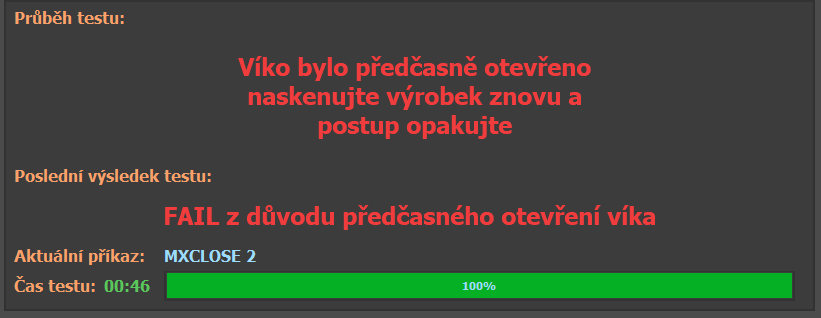
\includegraphics[height = 0.2\textheight]{obrazky/COVER_EDITED.PNG}
	\end{figure}

	V případě PASS a FAIL se nahraje výsledek do EMES (webová služba, kterou SIEMENS používá k ukládání dat)
    a podrobný log se uloží lokálně na cestu,
	která je odeslána do EMES a vytiskne se příslušný štítek.
	V případě FAIL z důvodu předčasného otevření víka nedojde k odeslání logu do EMES a Sériové číslo lze opět naskenovat.
	Poté je obsluha vyzvána k odebrání desky a naskenování nového kódu.

\end{enumerate}

\clearpage
\section{Paralelní programování}
Po naskenování určitých zakázek se program přepne do paralelního módu.
V tomto módu je možné naskenovat více sériových čísel a programovat tak DUT ve více pozicích najednou. Obsluha je instruována následovně:\\
\subsection{Skenování pozice A:}
V tomto bodě je obsluha k naskenování sériového čísla odpovídající DUT, které se bude zakládat do \mbox{pozice A.}
	\begin{figure}[ht!]
		\centering
		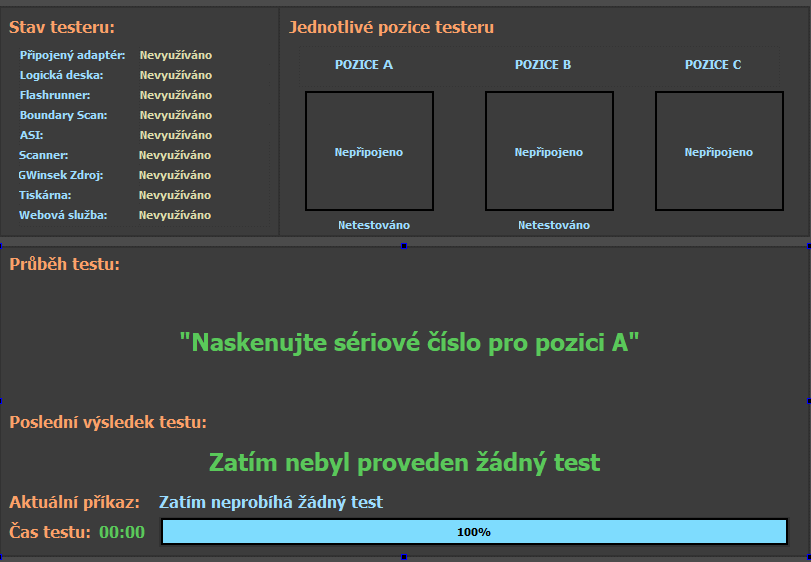
\includegraphics[height = 0.22\textheight]{obrazky/dual_SCAN_A.PNG}
        \caption{Skenování pozice A}
	\end{figure}

\subsection{Skenování pozice B:}
	V tomto bodě je obsluha vyzvána k naskenování sériového čísla odpovídající DUT, které se bude zakládat do pozice B. V případě,
	že obsluha chce otestovat pouze DUT v pozici A, může tento krok přeskočit a přímo vložit DUT do pozice A a zavřít víko.
	Po zavření víka je automaticky zkontrolováno, zda je DUT opravdu založeno do pozice A a začne test.
    Zároveň je obsluha graficky informována v části "jednotlivé pozici testeru"
    o stavu jednotlivých pozic. Grafické vyhodnocení je obdobné jako při neparalelním programování
    v sekci "Vložení desky do správné pozice".
	\begin{figure}[ht!]
		\centering
		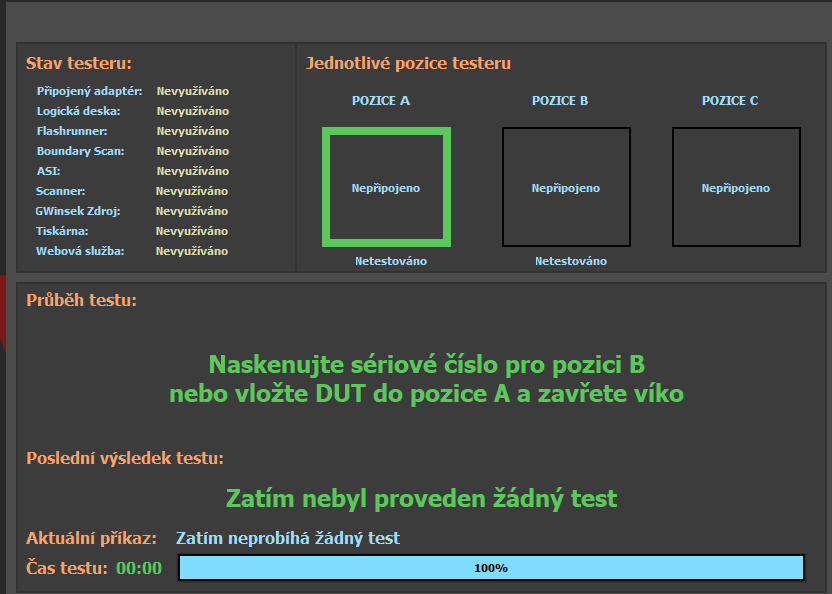
\includegraphics[height = 0.22\textheight]{obrazky/dual_SCAN_B.PNG}
        \caption{Skenování pozice A}
	\end{figure}


\subsection{Průběh testu:}
Po úspěšném založení DUT a zavření víka se spustí jednotlivé testy. Zároveň se změní popisky v části "Jednotlivé pozice testeru"\ následovně:
	\begin{figure}[ht!]
		\centering
		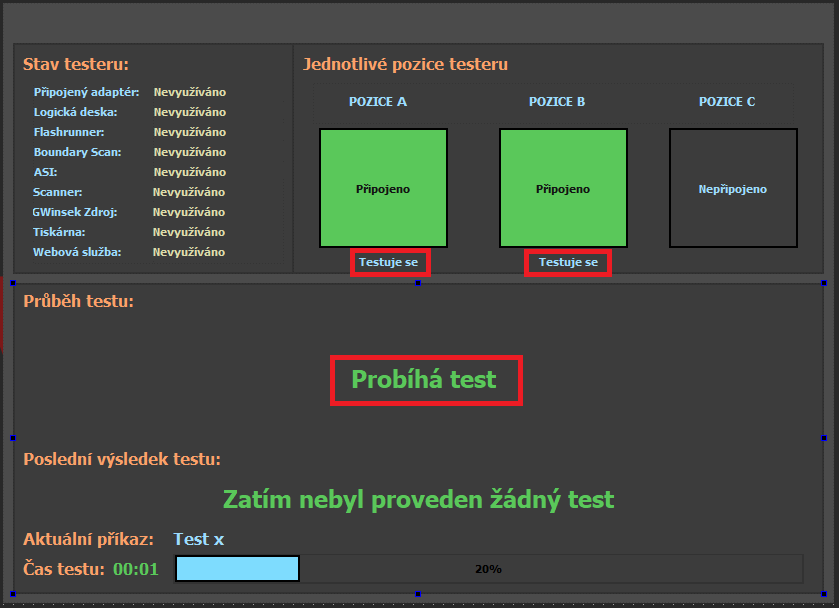
\includegraphics[height = 0.35\textheight]{obrazky/dual_SCAN_TEST.PNG}
        \caption{Průběh testu - paralelní programování}
	\end{figure}

\subsection{Výsledky testů:}
Výsledek testů je pak zobrazen pro jednotlivé pozice jak v části "Jednotlivé pozice testeru", tak v části "Průběh testu".
	\begin{figure}[ht!]
        \begin{minipage}{0.49\textwidth}
        \centering
		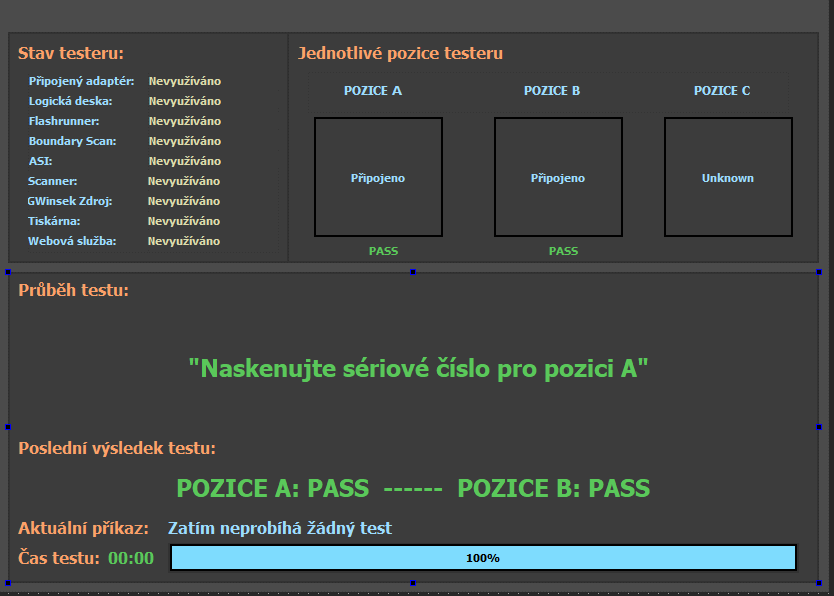
\includegraphics[height = 0.22\textheight]{obrazky/dual_SCAN_PASS.PNG}
        \caption{Výsledky testu - paralelní programování (PASS,PASS)}
        \end{minipage}
        \hfill
        \begin{minipage}{0.49\textwidth}
            \centering
            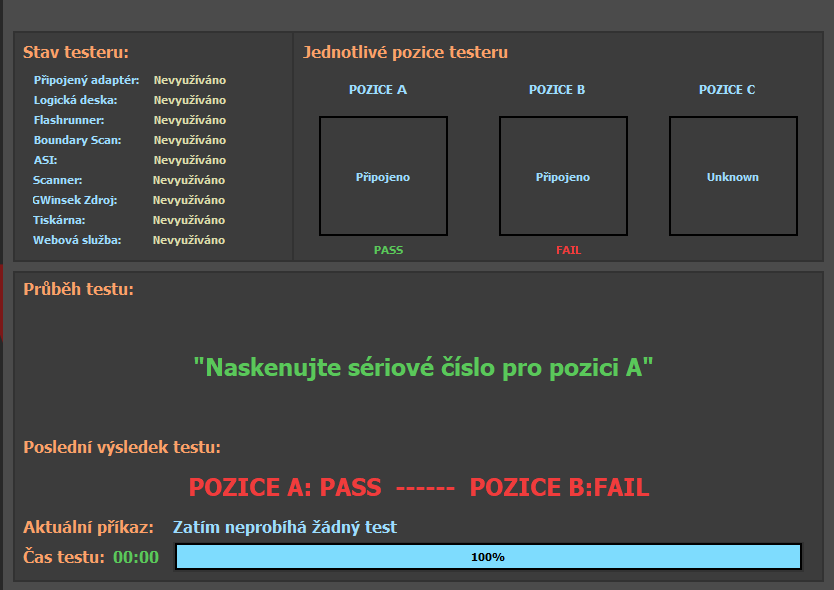
\includegraphics[height = 0.22\textheight]{obrazky/dual_SCAN_FAIL.PNG}
            \caption{Výsledky testu - paralelní programování (PASS,FAIL)}
            \end{minipage}
	\end{figure}


\clearpage
\section{Testování LED}
Pro některá DUT je implementováno manuální testování LED. V případě, že je takový test implementován, zobrazí
se obsluze následující dialog:
\begin{figure}[ht!]
	\centering
	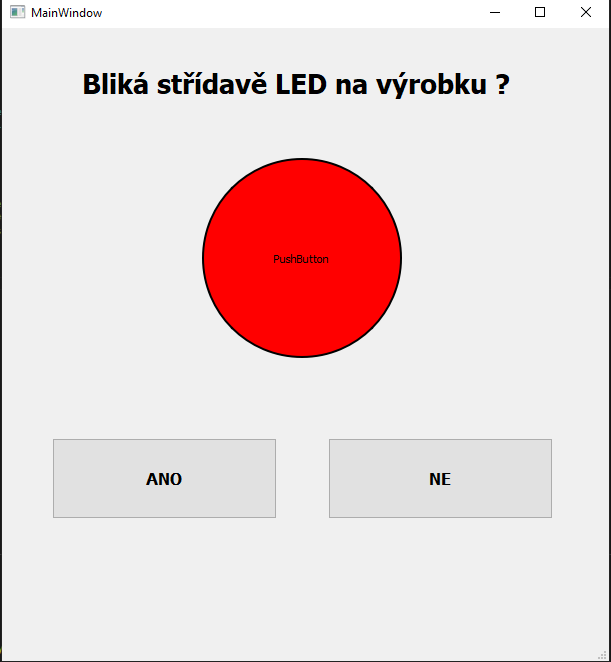
\includegraphics[width = 0.65\textwidth]{obrazky/LED_test.PNG}
    \caption{Testování LED}
\end{figure}

Obsluha zkontroluje, zda blikají/svítí příslušné LED a výsledek testu potvrdí kliknutím na tlačítko ANO popř. NE.
\clearpage

\chapter{Software - Administrátorský mód}

\textbf{\color{red} UPOPOZORNĚNÍ!!!\\
 Při používání softwaru v módu ADMIN nenese ČEVOR, spol. s r.o. žádnou odpovědnost za případné vzniklé škody spojené
s využíváním softwaru v tomto módu. Uživatel (Administrátor) tak přebírá plnou zodpovědnost za případné škody.}

Po přihlášení uživatele s oprávněním ADMIN se odemkne část ADMINISTRÁTORSKÉ MOŽNOSTI.
Aby bylo možné provádět jakékoliv akce v této sekci je nutné zaškrtnout políčko "Přepnout se do Admin. Prostředí".
Po přepnutí se do admin prostředí zobrazí ve vrchní části text pozastaveno a neprobíhá tak žádné testování.
Toto pole není možné zaškrtnout v případě, že již probíhá test.
Pokud se chcete vrát zpět do normálního módu testování políčko opět odškrtněte.
\begin{figure}[ht!]
	\centering
	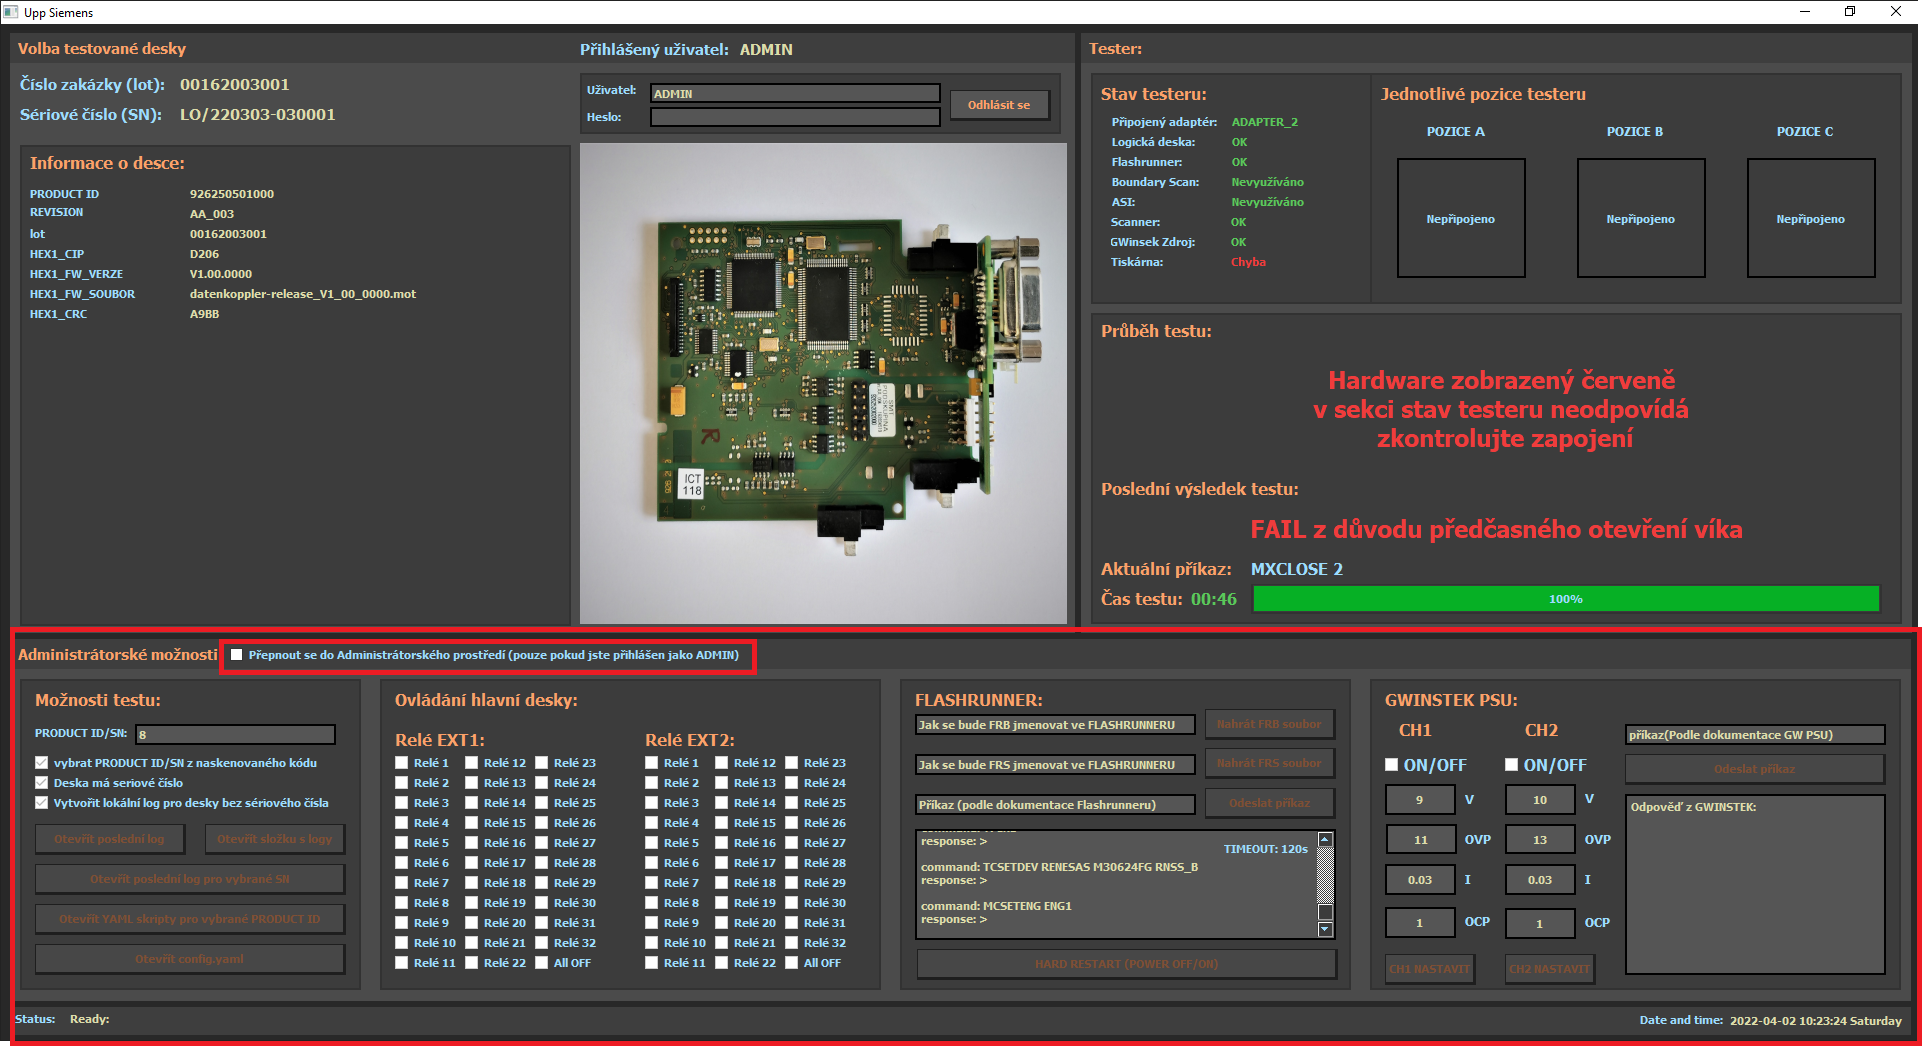
\includegraphics[width = 1\textwidth]{obrazky/ADMIN_edited.png}
    \caption{Odemčení administrátorského prostředí}
\end{figure}




\subsection{Sekce Možnosti testu:}
V případě, že deska nemá sériové číslo,
je zde možné povolit spuštění test bez naskenovaného SN.
Tuto možnost lze aktivovat odškrtnutím políčka "deska má sériové číslo".
Dále jsou zde tlačítka pro snazší otevírání složek a souborů s logy popř.
souborů popsaných v sekci "Struktura složek na konci dokumentu". 


\subsection{Sekce ovládání hlavní desky:}
Zde je možné přepínat jednotlivá relé na relé kartách v právě připojeném ADAPTÉRU.
\textbf{\color{red} NEVHODNÝM PŘEPNUTÍM RELÉ VŠAK MŮŽE DOJÍT K DESTRUKCI NĚKTERÝCH ZAŘÍZENÍ.}
Zapojení Relé karet lze najít ve schématu el. zapojení. 

\subsection{Sekce FLASHRUNNER:}
V této sekci je možné komunikovat s FLASHRUNNEREM pomocí zpráv komunikačního protokolu, který je popsán
v dataseheetu FLASHRUNNERU.
Dále je zde možné odesílat FRB a FRS soubory bez nutnosti vydělávání SD karet.

\subsection{Sekce GWINSTEK PSU:}
V této sekci je možné ovládat programovatelný zdroj GWINSTEK GPP-2323.
Jsou zde přednastaveny pole pro nastavování základních hodnot napětí a proudů.
Pro rozšířené možnosti lze využít pole v pravé části a posílat do programovatelného
zdroje příkazy podle datasheetu pro GWINSTEK GPP-2323

\section{Chyby}
V případě chybových hlášek zobrazených v části 3.
Se zkuste odhlásit odebráním karty a znovu přihlásit.
Po opakovaném přihlášení se může stát, že se zobrazí chybová hláška: ARRIGO neodpovídá.
V tomto případě zkuste počkat 40 až 60 sec. Tester totiž provádí po opětovném přihlášení sebekontrolu,
která může chvíli trvat. Pokud se chybová hláška neodstraní ani po uplynulé čekací době zkusit software restartovat.
V případě, že chybová hláška není odstraněna kontaktujte povolanou osobu. Například chyba z důvodu špatného připojení
tiskárny může vypadat takto:
\begin{figure}[ht!]
	\centering
	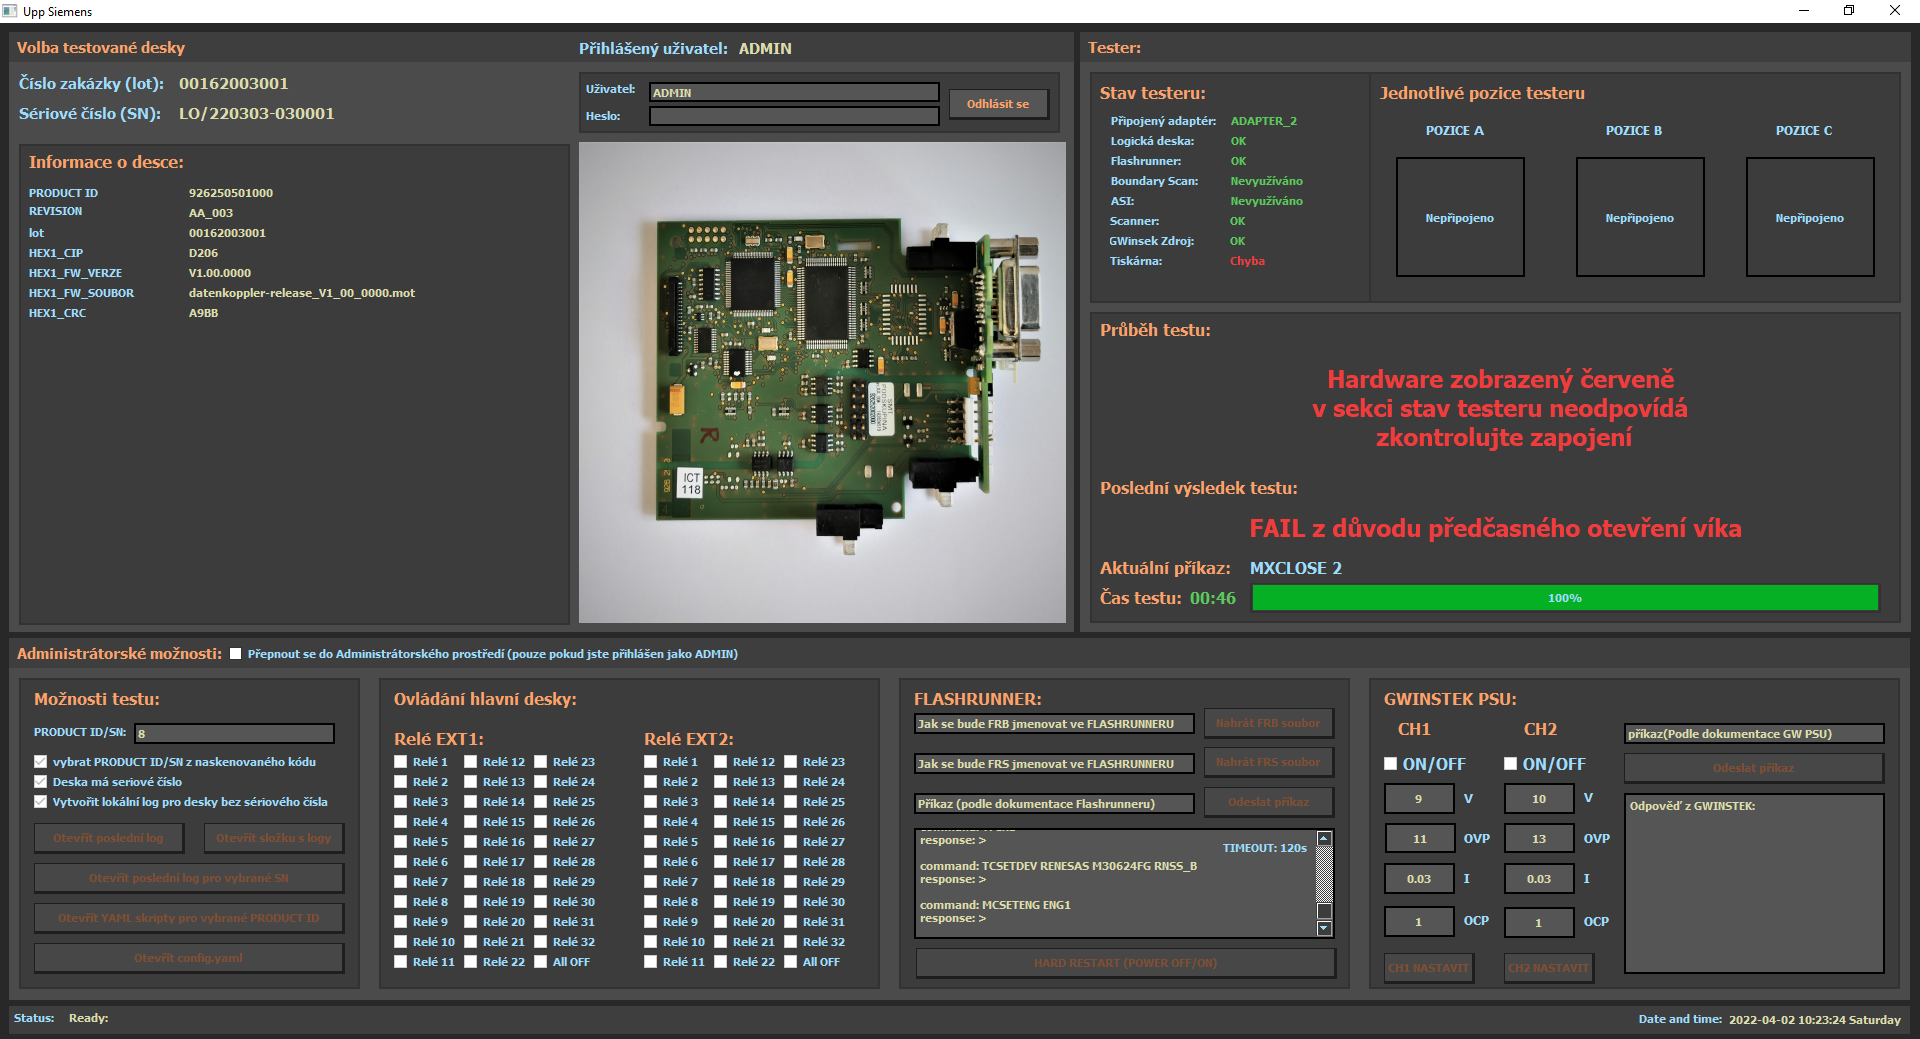
\includegraphics[width = 1\textwidth]{obrazky/HW_FAULT.PNG}
    \caption{chybová hláška z důvodu špatného připojení tiskárny}
\end{figure}



\clearpage
\chapter{Struktura složek:}
SOFTWARE lze konfigurovat pomocí souboru config.yaml.
Zde je možné měnit konfiguraci veškerého připojeného hardwaru, cestu k ukládaným logům,
WSDL k EMES atd.
Tento soubor také obsahuje postup testovacích procedur pro každé DUT v závislosti na "Material Number" s předponou P.
Pro větší přehlednost lze v každém testu volat vnořený yaml script,
který obsahuje skript s příkazy definovanými v datasheetu pro FLASHRUNNER.
Tyto příkazy jsou však upraveny tak, aby odpovídaly syntaxi .yaml souborům
(Obr.\ref{fig:Útržky ze souboru config.yaml}).

\begin{figure}[ht!]
	\centering
	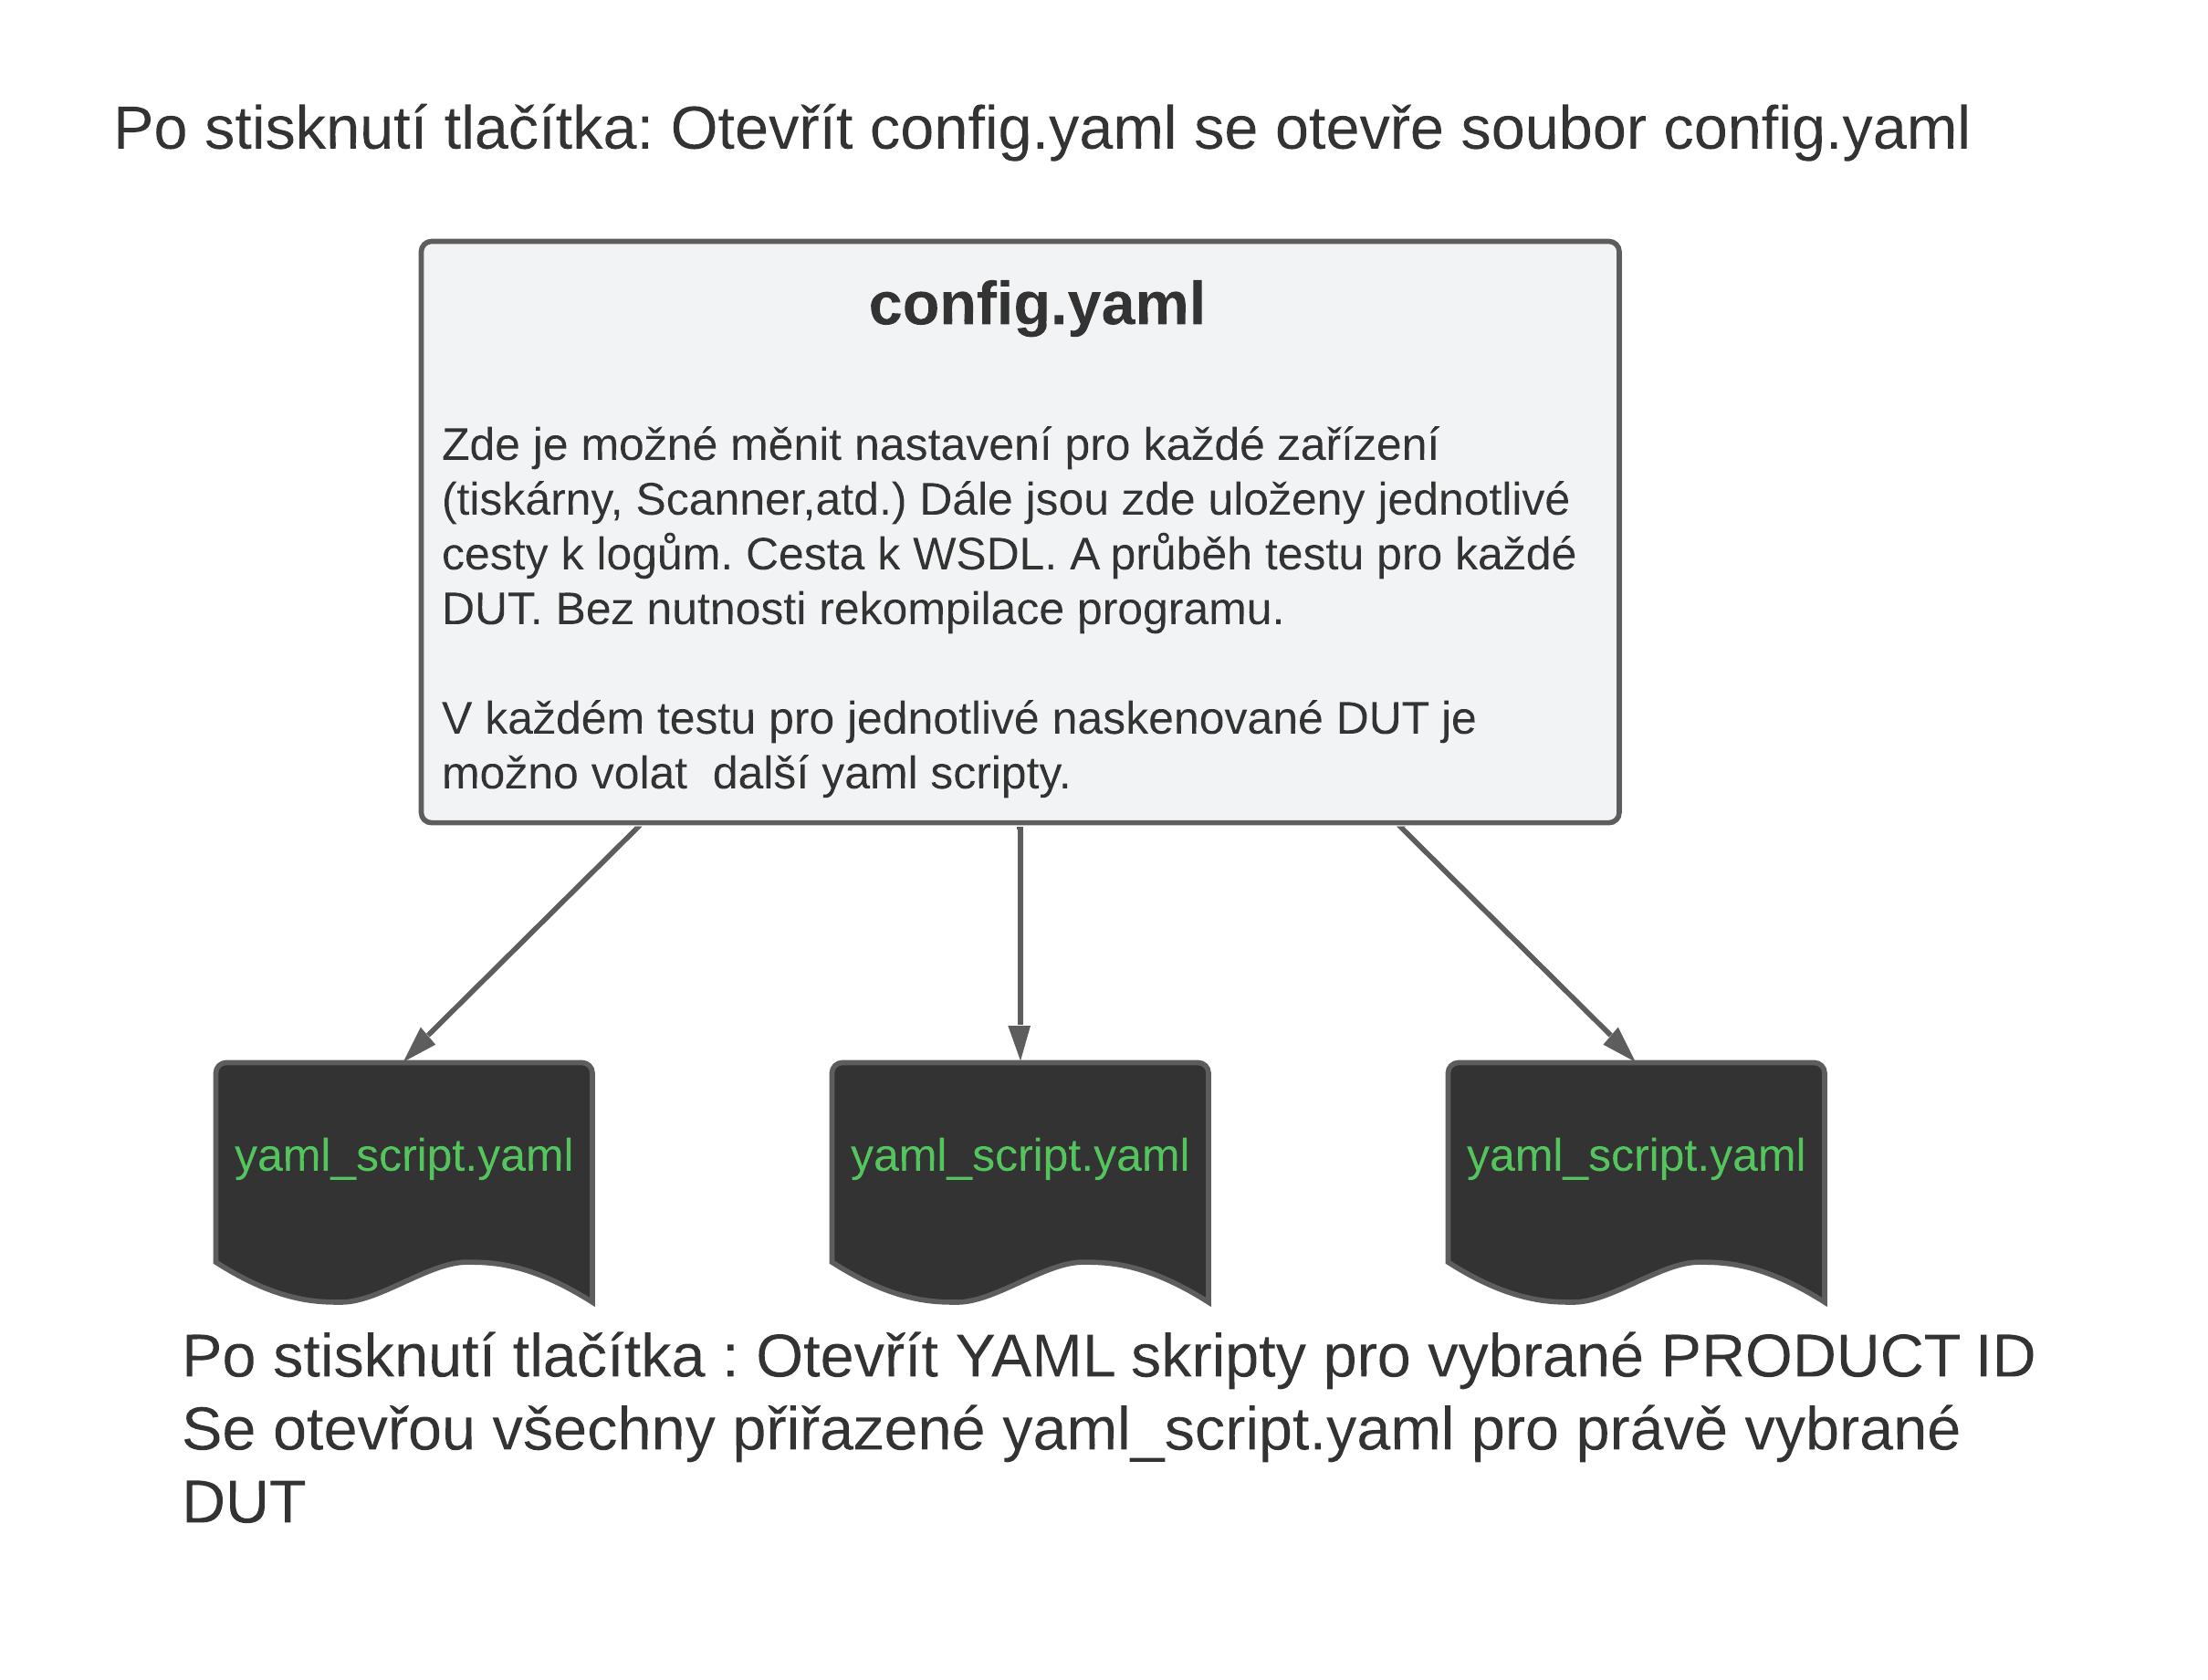
\includegraphics[width = 0.5\textwidth]{obrazky/Folder_diag.png}
    \caption{Struktura složek}
    
\end{figure}

Na následujícím  obrázku jsou útržky ze souboru config.yaml, kde je příklad pro nastavení WSDL a průběhu testu pro DUT,
které má material number 926251703000.
V STEP3 se zavolá script uložený na cestě:\\
\mbox{C:\/Users\/prod\_admin\/Desktop\/UPP\_refactor\/YAML\_SCRIPTS\/926257702000\_ATMEGA325.yaml}.\\
V tomto scriptu jsou dvě části INIT\_FR a MAIN. Tyto části budou volány postupně podle pořadí v jakém jsou napsány v souboru config.yaml. 

\begin{figure}[ht!]
	\centering
	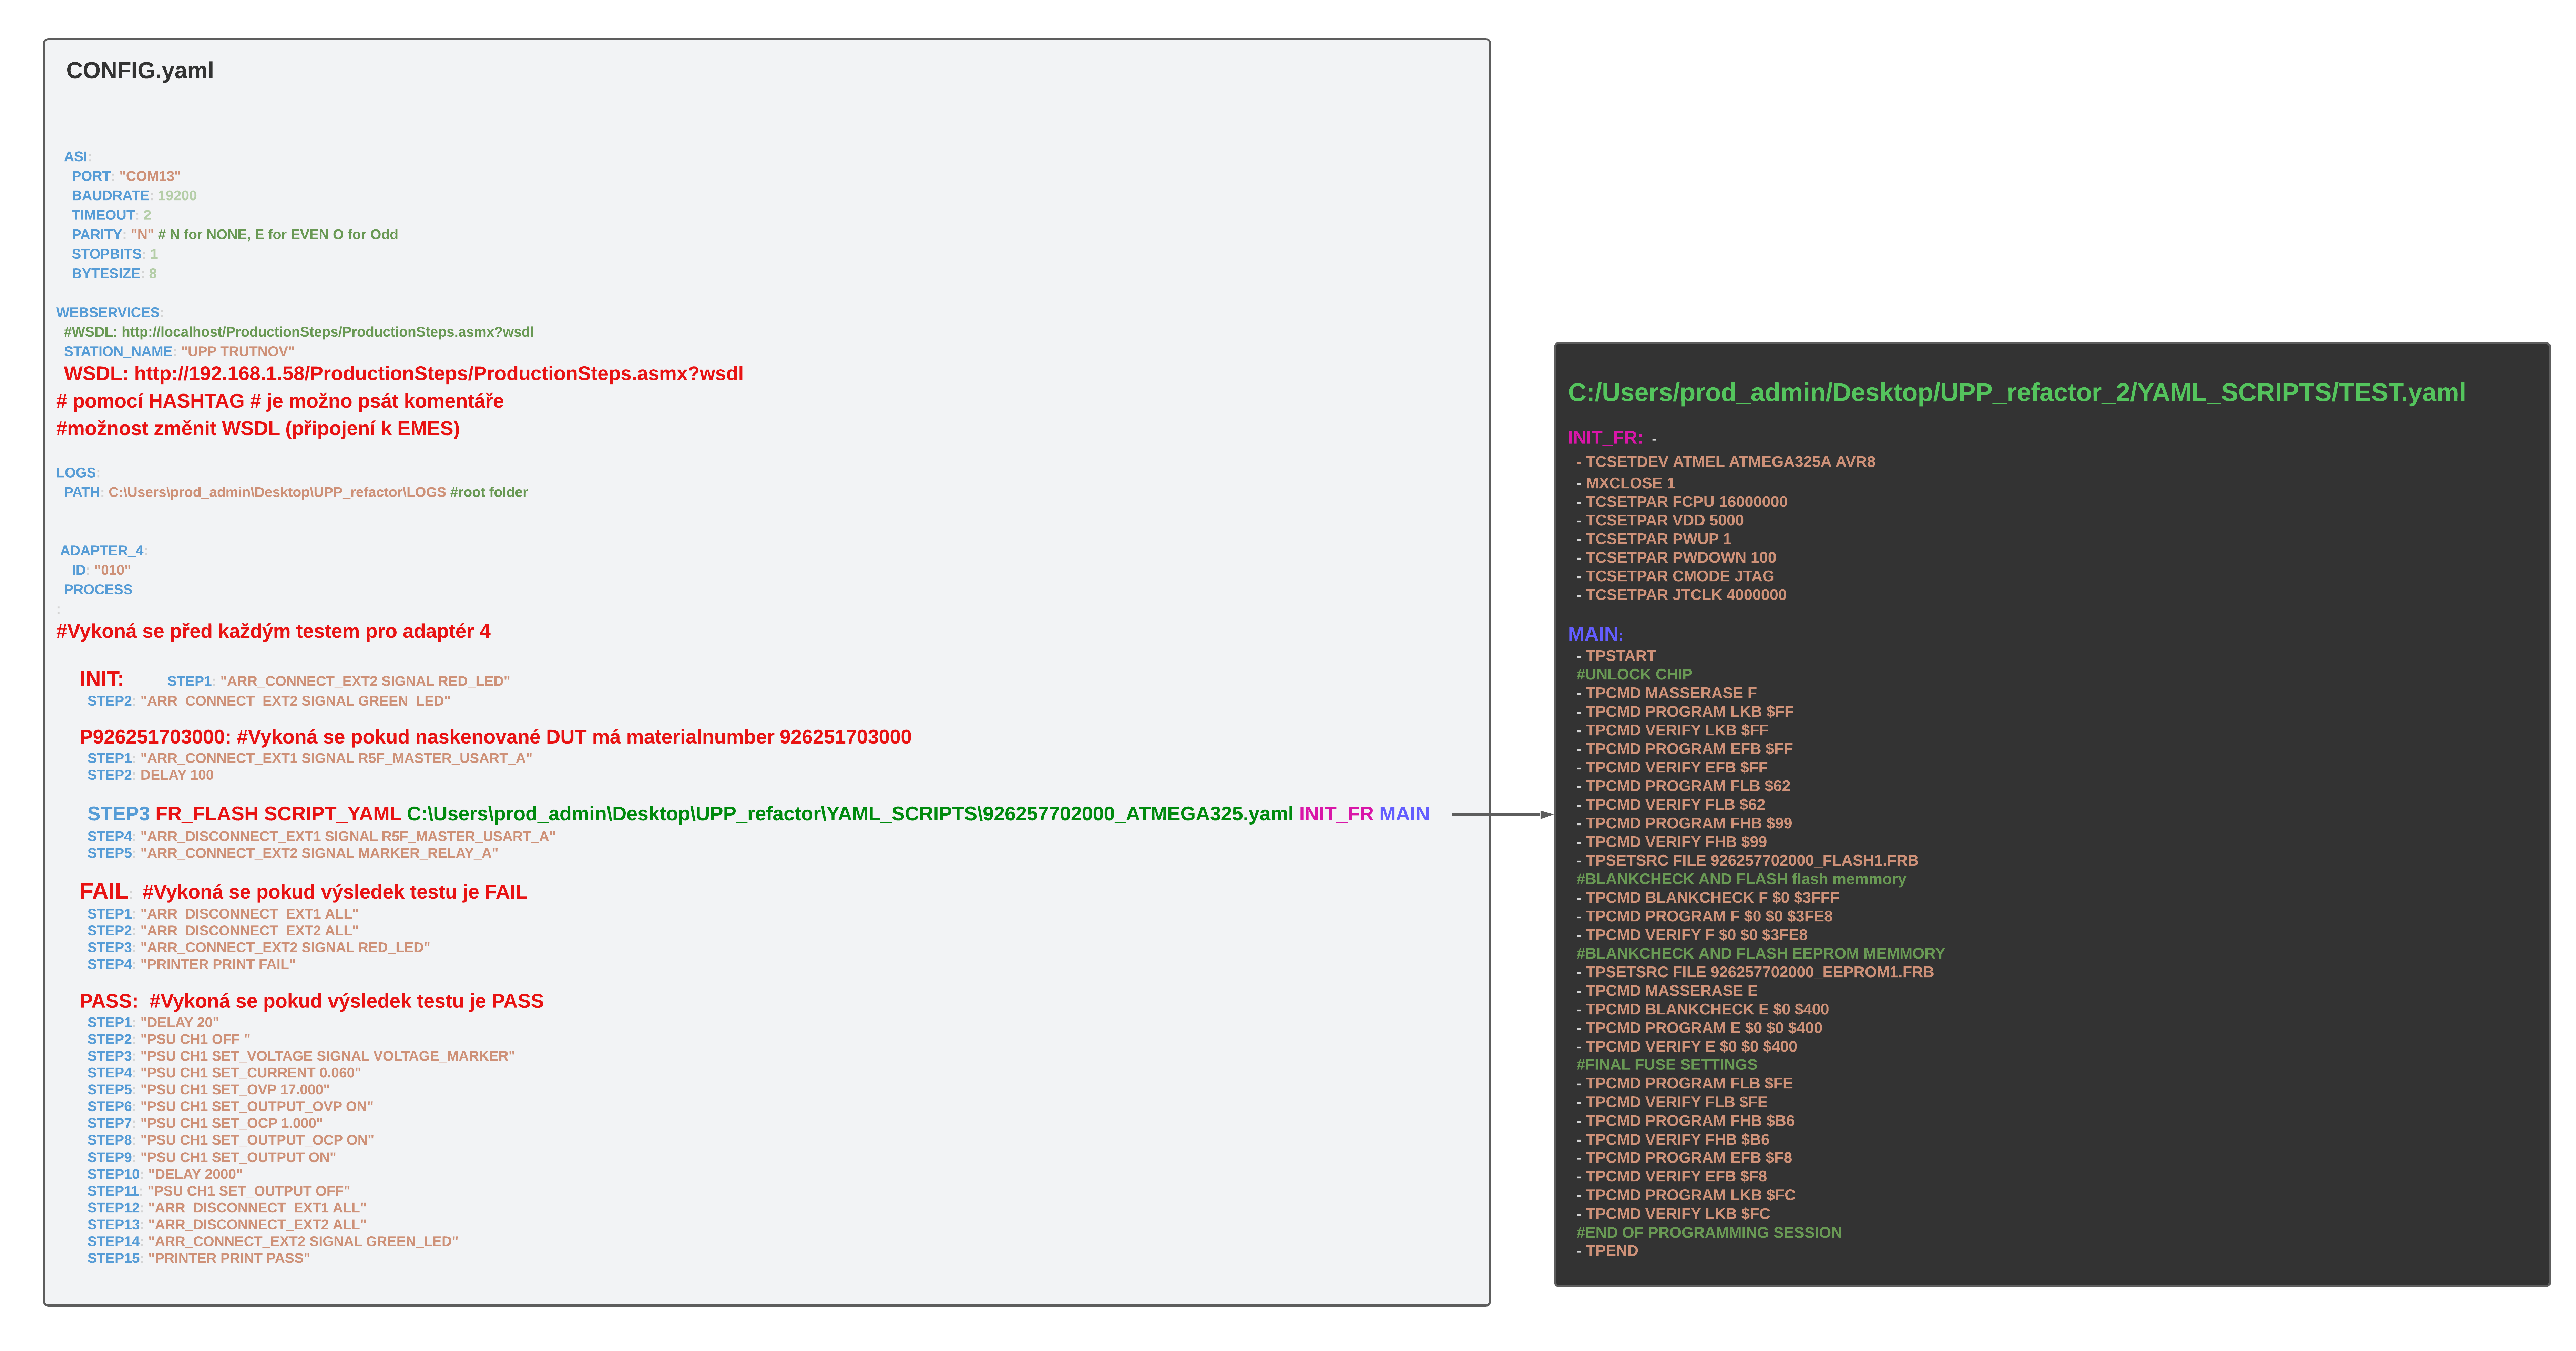
\includegraphics[width = 1\textwidth]{obrazky/FOLDER_TEXT.png}
    \caption{Útržky ze souboru config.yaml}
    \label{fig:Útržky ze souboru config.yaml}
\end{figure}

Je tak možné zavolat například pouze část INIT\_FR smazáním "MAIN"\ ze souboru config.yaml.
Následující příkaz bez volání MAIN sekce z .yaml scriptu by pak vypadal následovně:\\
STEP3: FR\_FLASH C:/.../YAML\_SCRIPTS/926257702000\_ATMEGA325.yaml INIT\_FR

\section{Přídavné utility}
 Softwarový balíček nabízí celou řadu utilit pro snadnější konfiguraci a údržbu testeru.
 Jedná se například o programy umožňující nastavovat správnou syntaxi yaml scriptů, jednodušší procházení logů,
 testování jednotlivých částí testeru bez nutnosti připojení do EMES, přímou komunikaci s programátory,
 ovládání značkovačů (frézek), testování EMES, simulace TCP/IP serveru pro přihlašování pomocí karet, debugování apod.


\chapter*{Závěr}
\phantomsection
\addcontentsline{toc}{chapter}{Závěr}

Výsledkem odborné praxe je realizace univerzálního programovacího pracoviště.
Kromě své hardwarové části je k pracovišti vytvořena softwarová platforma, která
umožňuje relativně jednoduchou úpravu a rozšiřování funkčnosti.\\

K pracovišti byla vytvořena kompletní dokumentace k elektrické, mechanické a softwarové části.
Přičemž práce studenta byla zaměřena převážně na elektrickou a softwarovou část.
Dále byla vytvořena analýza rizik, předpis údržby a další předávací protokoly.\\

V současné době je pracoviště ve výrobním provozu firmy SIEMENS a postupně se 
rozšiřuje o další funkce a adaptéry.
Během dosavadního provozu bylo odhaleno několik chyb a nedostatků, které se postupně odstraňují.
Hlavním přínosem práce (kromě finanční odměny) je vytvoření softwarové platformy pro jednoduché propojování
různých zařízení.\\

\section*{Poděkování}
Závěrem bych chtěl poděkovat odbornému vedoucímu práce Radomilu Havlínovi. Jsem velmi rád,
že mi umožnil vést tento 3 týdenní až roční projekt.
Jeho revírem jsou revize,
Jeho tempo bylo vražedné, našimi 
protivníky byly korporátní schůzky, nefunkční hardware a nedostatek času.
Byl v nasazení ve dne, v noci a jeho úkolem je zajistit bezpečnost. Děkuji.

\vfill
\begin{flushright}
\begin{tabular}{@{}p{2.5in}@{}}
\hrulefill \\
Vedoucí práce \\
Ing. Radomil Havlín
\end{tabular}
\end{flushright}


\end{document}
